% A LaTeX template for ARTICLE version of the MSc Thesis submissions to 
% Politecnico di Milano (PoliMi) - School of Industrial and Information Engineering
%
% S. Bonetti, A. Gruttadauria, G. Mescolini, A. Zingaro
% e-mail: template-tesi-ingind@polimi.it
%
% Last Revision: October 2021
%
% Copyright 2021 Politecnico di Milano, Italy. Inc. NC-BY

\documentclass[11pt,a4paper]{article} 

%------------------------------------------------------------------------------
%	REQUIRED PACKAGES AND  CONFIGURATIONS
%------------------------------------------------------------------------------
% PACKAGES FOR TITLES
\usepackage{titlesec}
\usepackage{color}

% PACKAGES FOR LANGUAGE AND FONT
\usepackage[utf8]{inputenc}
\usepackage[english]{babel}
\usepackage[T1]{fontenc} % Font encoding

% PACKAGES FOR IMAGES
\usepackage{graphicx}
\usepackage[utf8]{inputenc}
\graphicspath{{Images/}}
\usepackage{eso-pic} % For the background picture on the title page
\usepackage{caption} % Coloured captions
\usepackage{transparent}

% STANDARD MATH PACKAGES
\usepackage{amsmath}
\usepackage{amsthm}
\usepackage{bm}
\usepackage[overload]{empheq}  % For braced-style systems of equations

% PACKAGES FOR TABLES
\usepackage{tabularx}
\usepackage{longtable} % tables that can span several pages
\usepackage{colortbl}

% PACKAGES FOR ALGORITHMS (PSEUDO-CODE)
\usepackage{algorithm}
\usepackage{algorithmic}

% PACKAGES FOR REFERENCES & BIBLIOGRAPHY
\usepackage[colorlinks=true,linkcolor=black,anchorcolor=black,citecolor=black,filecolor=black,menucolor=black,runcolor=black,urlcolor=black]{hyperref} % Adds clickable links at references
\usepackage{cleveref}
\usepackage[square, numbers, sort&compress]{natbib} % Square brackets, citing references with numbers, citations sorted by appearance in the text and compressed
\bibliographystyle{plain} % You may use a different style adapted to your field

\usepackage{hyperref} % for adding links

% PACKAGES FOR THE APPENDIX
\usepackage{appendix}

% PACKAGES FOR ITEMIZE & ENUMERATES 
\usepackage{enumitem}

% OTHER PACKAGES
\usepackage{amsthm,thmtools,xcolor} % Coloured "Theorem"
\usepackage{comment} % Comment part of code
\usepackage{fancyhdr} % Fancy headers and footers
\usepackage{lipsum} % Insert dummy text
\usepackage{tcolorbox} % Create coloured boxes (e.g. the one for the key-words)
\usepackage{amsmath}
\usepackage{amssymb}

\usepackage{minted}
\usepackage{subcaption}



%-------------------------------------------------------------------------
%	NEW COMMANDS DEFINED
%-------------------------------------------------------------------------
% EXAMPLES OF NEW COMMANDS -> here you see how to define new commands
\newcommand{\bea}{\begin{eqnarray}} % Shortcut for equation arrays
\newcommand{\eea}{\end{eqnarray}}
\newcommand{\e}[1]{\times 10^{#1}}  % Powers of 10 notation
\newcommand{\mathbbm}[1]{\text{\usefont{U}{bbm}{m}{n}#1}} % From mathbbm.sty
\newcommand{\pdev}[2]{\frac{\partial#1}{\partial#2}}
% NB: you can also override some existing commands with the keyword \renewcommand

%----------------------------------------------------------------------------
%	ADD YOUR PACKAGES (be careful of package interaction)
%----------------------------------------------------------------------------


%----------------------------------------------------------------------------
%	ADD YOUR DEFINITIONS AND COMMANDS (be careful of existing commands)
%----------------------------------------------------------------------------


% Do not change Configuration_files/config.tex file unless you really know what you are doing. 
% This file ends the configuration procedures (e.g. customizing commands, definition of new commands)
% Configuration package
\usepackage[bottom=2.0cm,top=2.0cm,left=2.0cm,right=2.0cm]{geometry}
\raggedbottom 

% Create color bluePoli (-> manuale grafica coordinata:  https://www.polimi.it/fileadmin/user_upload/il_Politecnico/grafica-coordinata/2015_05_11_46xy_manuale_grafica_coordinata.pdf)
\definecolor{bluePoli}{cmyk}{0.4,0.1,0,0.4}

% Custom theorem environments
\declaretheoremstyle[
  headfont=\color{bluePoli}\normalfont\bfseries,
  bodyfont=\color{black}\normalfont\itshape,
]{colored}

\captionsetup[figure]{labelfont={color=bluePoli}} % Set colour of the captions
\captionsetup[table]{labelfont={color=bluePoli}} % Set colour of the captions
\captionsetup[algorithm]{labelfont={color=bluePoli}} % Set colour of the captions

\theoremstyle{colored}
\newtheorem{theorem}{Theorem}[section]
\newtheorem{proposition}{Proposition}[section]

% Enhances the features of the standard "table" and "tabular" environments.
\newcommand\T{\rule{0pt}{2.6ex}}
\newcommand\B{\rule[-1.2ex]{0pt}{0pt}}

% Algorithm description
\newcounter{algsubstate}
\renewcommand{\thealgsubstate}{\alph{algsubstate}}
\newenvironment{algsubstates}{
    \setcounter{algsubstate}{0}%
    \renewcommand{\STATE}{%
    \stepcounter{algsubstate}%
    \Statex {\small\thealgsubstate:}\space}
    }{}
    
% Custom theorem environment
\newcolumntype{L}[1]{>{\raggedright\let\newline\\\arraybackslash\hspace{0pt}}m{#1}}
\newcolumntype{C}[1]{>{\centering\let\newline\\\arraybackslash\hspace{0pt}}m{#1}}
\newcolumntype{R}[1]{>{\raggedleft\let\newline\\\arraybackslash\hspace{0pt}}m{#1}}

% Custom itemize environment
\setlist[itemize,1]{label=$\bullet$}
\setlist[itemize,2]{label=$\circ$}
\setlist[itemize,3]{label=$-$}
\setlist{nosep}

% Create command for background pic
\newcommand\BackgroundPic{% Adding background picture
	\put(237,365){
	    \parbox[b][\paperheight]{\paperwidth}{%
	    \vfill
		\centering
		\transparent{0.4}
		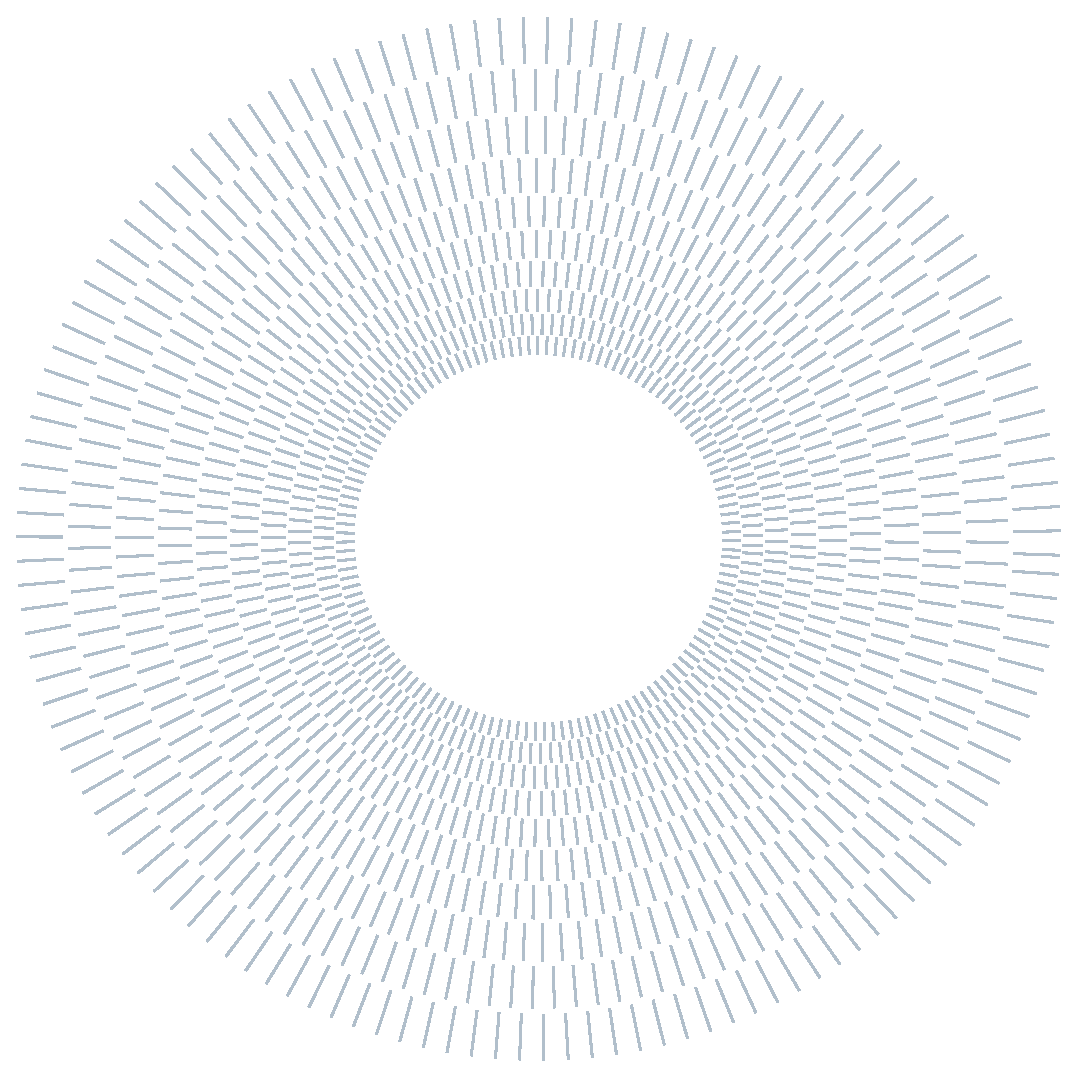
\includegraphics[width=0.44\paperwidth]{raggiera_polimi.eps}%
		\vfill}
		}
}

% Set indentation
\setlength\parindent{0pt}

% Custom title commands
\titleformat{\section}
{\color{bluePoli}\normalfont\Large\bfseries}
{\color{bluePoli}\thesection.}{1em}{}
\titlespacing*{\section}
{0pt}{3.3ex}{3.3ex}

\titleformat{\subsection}
{\color{bluePoli}\normalfont\large\bfseries}
{\color{bluePoli}\thesubsection.}{1em}{}
\titlespacing*{\subsection}
{0pt}{3.3ex}{3.3ex}

% Custom headers and footers
\pagestyle{fancy}
\fancyhf{}
      
\fancyfoot{}
\fancyfoot[C]{\thepage} % page
\renewcommand{\headrulewidth}{0mm} % headrule width
\renewcommand{\footrulewidth}{0mm} % footrule width

\makeatletter
\patchcmd{\headrule}{\hrule}{\color{black}\hrule}{}{} % headrule
\patchcmd{\footrule}{\hrule}{\color{black}\hrule}{}{} % footrule
\makeatother

% Insert here the info that will be displayed into your Title page 
% -> title of your work
\renewcommand{\title}{Randomized Linear Algebra and its Applications}
% -> author name and surname
\renewcommand{\author}{Jasmin Spinetto, Peng Rao, Anna Paola Izzo, Cao Wu, Jiali Claudo Haung}
% -> MSc course
\newcommand{\course}{High Performance Computing Engineering - Advanced Methods for Scientific Computing}
% -> advisor name and surname
\newcommand{\advisor}{Prof. Luca Formaggia}
% IF AND ONLY IF you need to modify the co-supervisors you also have to modify the file Configuration_files/title_page.tex (ONLY where it is marked)
%\newcommand{\firstcoadvisor}{Name Surname} % insert if any otherwise comment
% -> author ID
\newcommand{\ID}{\\10734813, 11022931, 10680171, 11036000, 11032111}
% -> academic year
\newcommand{\YEAR}{2024-2025}
% -> abstract (only in English)
\renewcommand{\abstract}{In this work, we present an efficient implementation of the randomized Singular Value Decomposition (rSVD) algorithm, along with its parallelized versions and a benchmarking analysis. Our study explores the performance and scalability of these implementations, demonstrating their advantages in handling large-scale datasets. To show the practical applications of rSVD, we apply it to three key concrete problems: image compression, handwritten number recognition, and Principal Component Analysis (PCA), providing quantitative results that highlight their effectiveness. Additionally, we implement the CUR decomposition algorithm, both in its deterministic and randomized versions, as an alternative low-rank approximation method. We also analyzed its performance with respect to SVD. Our findings underscore the computational benefits of randomized techniques and their potential for real-world applications.}

% -> key-words (only in English)
\newcommand{\keywords}{Randomized Linear Algebra, RandomizedSVD, CUR Decomposition, Applications}

%-------------------------------------------------------------------------
%	BEGIN OF YOUR DOCUMENT
%-------------------------------------------------------------------------
\begin{document}

%-----------------------------------------------------------------------------
% TITLE PAGE
%-----------------------------------------------------------------------------
% Do not change Configuration_files/TitlePage.tex (Modify it IF AND ONLY IF you need to add or delete the Co-advisors)
% This file creates the Title Page of the document
% DO NOT REMOVE SPACES BETWEEN LINES!

\AddToShipoutPicture*{\BackgroundPic}

\hspace{-0.6cm}
\includegraphics[width=0.6\textwidth]{logo_polimi_ing_indinf.eps}

\vspace{-1mm}
\Large{\textbf{\color{bluePoli}{\title}}}\\

\vspace{-0.2cm}
\fontsize{0.3cm}{0.5cm}\selectfont \bfseries \textsc{\color{bluePoli} \course}\\

\vspace{-0.2cm}
\normalfont{\textbf{\author, \ID}}

\small \normalfont

\vspace{11pt}

\centerline{\rule{1.0\textwidth}{0.4pt}}

\begin{center}
\begin{minipage}[t]{.24\textwidth}
\begin{minipage}{.90\textwidth}
\noindent
\scriptsize{\textbf{Advisor:}} \\
\advisor \\
\\
% \textbf{Co-advisors:} \\ % leave it if any co-advisor otherwise comment
% \firstcoadvisor \\ % leave it if any co-advisor otherwise comment
% \secondcoadvisor \\ % leave it if you have more that one co-advisor otherwise comment (if you have more than two co-advisors just copy&paste this line writing \thirdcoadvisor, \fourthcoadvisor, ecc. (REMEMBER to modify also the main.txt)
\\ % leave it if any co-advisor otherwise comment
\textbf{Academic year:} \\
\YEAR \\
\\
\end{minipage}
\end{minipage}% This must go next to `\end{minipage}`
\begin{minipage}{.74\textwidth}
\noindent \textbf{\color{bluePoli} Abstract:} {\abstract}
\end{minipage}
\end{center}

\vspace{15pt}

\begin{tcolorbox}[arc=0pt, boxrule=0pt, colback=bluePoli!60, width=\textwidth, colupper=white]
    \textbf{Key-words:} \keywords
\end{tcolorbox}

\vspace{12pt}

%-----------------------------------------------------------------------------
% INTRODUCTION
%-----------------------------------------------------------------------------
\section{Introduction}
In this project we developed a custom implementation of the \textbf{Randomized Singular Value Decomposition (rSVD)} algorithm in C++ and conducted a benchmarking to compare its performance with the \texttt{BDCSVD} implementation provided by the \texttt{Eigen} library. Furthemore, we explored some \textbf{concrete application cases} of the RandomizedSVD decomposition method as:
\begin{itemize}
    \item Image Compression
    \item Handwritten Numbers Recognition
    \item Principal Component Analysis
\end{itemize}
In addition to RSVD, we implemented and tested also the \textbf{CUR decomposition algorithm}, which is another randomized technique for approximating matrices, exploring both it's deterministic and randomized implementations.\\
This report outlines the theoretical background of RSVD and CUR decomposition, describes the implementation details of our algorithms and presents the results of our benchmarks and application experiments. Through this work, we aim to demonstrate the practical utility of randomized linear algebra techniques in solving computationally demanding problems while ensuring efficiency and accuracy. \\
The only pre-existing code utilized in our rSVD implementation was the matrix operations provided by the \textbf{Eigen library}, which facilitated efficient handling of matrix manipulations.

%-----------------------------------------------------------------------------
% EQUATIONS
%-----------------------------------------------------------------------------
\section{Randomized Linear Algebra}
Random Linear Algebra is a branch of mathematics that combines principles from linear algebra with techniques from probability and statistics to analyze and solve problems involving large-scale or high-dimensional data. The base idea is to introduce \textbf{randomness} into computations to make algorithms faster, simpler, more efficient, more scalable, or more robust while maintaining accurate approximations of the desired results. This is needed because traditional linear algebra techniques can become computationally expensive for large datasets, such as those encountered in machine learning, data science, and numerical simulations. Randomized algorithms help mitigate these challenges by:
\begin{itemize}
    \item Reducing computation complexity
    \item Lowering memory requirements
    \item Allowing for parallelization and distributed computing
\end{itemize}



The main techniques used are:
\begin{itemize}
    \item \textbf{Randomized Sampling}: instead of processing an entire matrix, Randomized Linear Algebra uses random sampling to approximate matrix operations. For example by:
    \begin{itemize}
    \item \textit{Row/column sampling}: selecting a subset of rows or columns from a matrix based on a probability distribution to approximate its structure.
    \item \textit{Sketching}: compressing a large matrix into a smaller one ("sketch matrix") while preserving key properties, such as norms or singular values.
    \end{itemize}
    \item \textbf{Low-Rank Approximation}: many large matrices encountered in practice are approximately low-rank, meaning their significant information can be captured by a smaller number of dimensions. Randomized techniques are used to compute these approximations efficiently:
    \begin{itemize}
        \item \textit{Randomized SVD (Singular Value Decomposition)}: Approximating the singular values and vectors using random projections.
        \item \textit{CUR Decomposition}: representing a matrix using a subset of its actual rows (C) and columns (R), and a smaller core matrix (U).
    \end{itemize}
    \item \textbf{Random Projections}: high-dimensional data can be projected into a lower-dimensional space using random matrices, such as Gaussian random matrices and Sparse random matrices.
    \item \textbf{Montecarlo methods}: randomized algorithms often rely on Monte Carlo methods to provide probabilistic guarantees about the accuracy of approximations. For example, the probability of achieving a given approximation error is often a parameter of the algorithm.
    \item \textbf{Stochastic Iterative Methods}: iterative solvers for linear systems, such as gradient descent, can be randomized by incorporating stochastic components, which often improves convergence rates or reduces computational cost in large-scale problems.
\end{itemize}

\subsection{Challenges}
The main challenges of using Randomized Linear Algebra lie in \textbf{balancing efficiency and accuracy}. Since RLA methods rely on approximations, they introduce a trade-off between computational speed and the precision of results, which may not be acceptable in highly sensitive applications. Additionally, the performance of these methods depends on how the parameters are tuned, such as sampling size and pattern or random projections choice. For example, in a randomized SVD decomposition, using less random samples (meaning a lower rank) reduced computation time but can cause missing important features of the matrix, leading to an inaccurate low-rank approximation. \\
\textbf{Randomized Linear Algebra can become ineffective} when it's applied to highly ill-conditioned or extremely sparse matrices, to data with outliers or heavy noise, or when it is used for highly sensitive applications or small-scale problems.

\pagebreak
\section{Randomized Singular Value Decomposition}
We have already implemented the following algorithms:
\begin{itemize}
    \item QR factorization using Given's rotation: \texttt{GivensRotation}
    \item Basic SVD using Power Method: \texttt{PowerMethod}
    \item Randomized singular value decomposition: \texttt{RandomizedSVD}
\end{itemize}
\subsection{QR Factorization}
The Givens Rotation Q R decomposition is a method for decomposing a matrix $A$ into an orthogonal matrix $Q$ and an upper triangular matrix $R$, such that:
\[
    A = Q R
\]
A Givens rotation matrix is used to zero out specific elements of a matrix. For two elements $a$ and $b$, the Givens rotation coefficients $c$ and $s$ are calculated such that:
\[
    \begin{bmatrix}
        c & s \\
        -s & c
    \end{bmatrix}
    \begin{bmatrix}
        a \\
        b
    \end{bmatrix}
    =
    \begin{bmatrix}
        r \\
        0
    \end{bmatrix}
\]
where $r = \sqrt{a^2 + b^2}$. The Givens rotation matrix is then used to zero out the element $b$ by multiplying the matrix from the left:
\[
    \begin{bmatrix}
        c  & s \\
        -s & c
    \end{bmatrix}
    \begin{bmatrix}
        a & b \\
        c & d
    \end{bmatrix}
    =
    \begin{bmatrix}
        r & 0  \\
        0 & d'
    \end{bmatrix}
\]
where $d' = c d - s b$. The Givens rotation matrix is a efficient way to perform QR decomposition, especially for sparse matrices. The pseudocode for the Givens rotation QR decomposition is shown in Algorithm \ref{alg:givens}.

\begin{algorithm}
\caption{Givens Rotation Algorithm}
\begin{algorithmic}[1]
\label{alg:givens}
\REQUIRE Matrix \( A \in \mathbb{R}^{m \times n} \), indices \( i, j \), and column \( k \) (\( 1 \leq i < j \leq m \))
\ENSURE Matrix \( A \) with the element \( A[j, k] \) eliminated
\STATE Compute \( r \gets \sqrt{A[i, k]^2 + A[j, k]^2} \)
\STATE Compute \( c \gets \frac{A[i, k]}{r} \) and \( s \gets \frac{A[j, k]}{r} \)
\FOR{\( l = k \) to \( n \)}
    \STATE \( t \gets A[i, l] \) \COMMENT{Temporary storage for row \( i \)}
    \STATE \( A[i, l] \gets c \cdot A[i, l] + s \cdot A[j, l] \)
    \STATE \( A[j, l] \gets -s \cdot t + c \cdot A[j, l] \)
\ENDFOR
\end{algorithmic}
\end{algorithm}

We implemented the Givens Rotation algorithm and utilized template metaprogramming techniques to achieve optimizations for both dense and sparse matrices. To construct this QR factorization solver, we can use both the following initializes:
\begin{minted}[fontsize=\small, linenos, frame=single]{cpp}
Eigen::GivensRotationQR<Eigen::MatrixXd> givens_rotation_qr; // for dense
Eigen::GivensRotationQR<Eigen::SparseMatrix<double>> givens_rotation_qr; // for sparse
\end{minted}
We conducted a benchmark of Algorithm \ref{alg:givens}, testing matrix sizes ranging from 100 $\times$ 100 to 1000 $\times$ 1000, and compared it with the \texttt{SparseQR} algorithm implemented in \texttt{Eigen}. And we also tested the computation results using \texttt{NumPy} with the same sparse matrices.. The results are presented in the following figure \ref{fig:qr_performance}.

Our implementation outperformed \texttt{SparseQR}, achieved results comparable to \texttt{NumPy}, and even slightly surpassed \texttt{NumPy} by approximately 5 to 20 times. Since \texttt{NumPy} is built on \texttt{OpenBLAS} at its core but is slower due to the Python language compared to C++, this result aligns with expectations. The results show that Givens rotation implementation is a competitive and efficient approach compared to the baseline.

\begin{figure}[H]
    \centering
    % left figure
    \begin{subfigure}[b]{0.48\textwidth}
        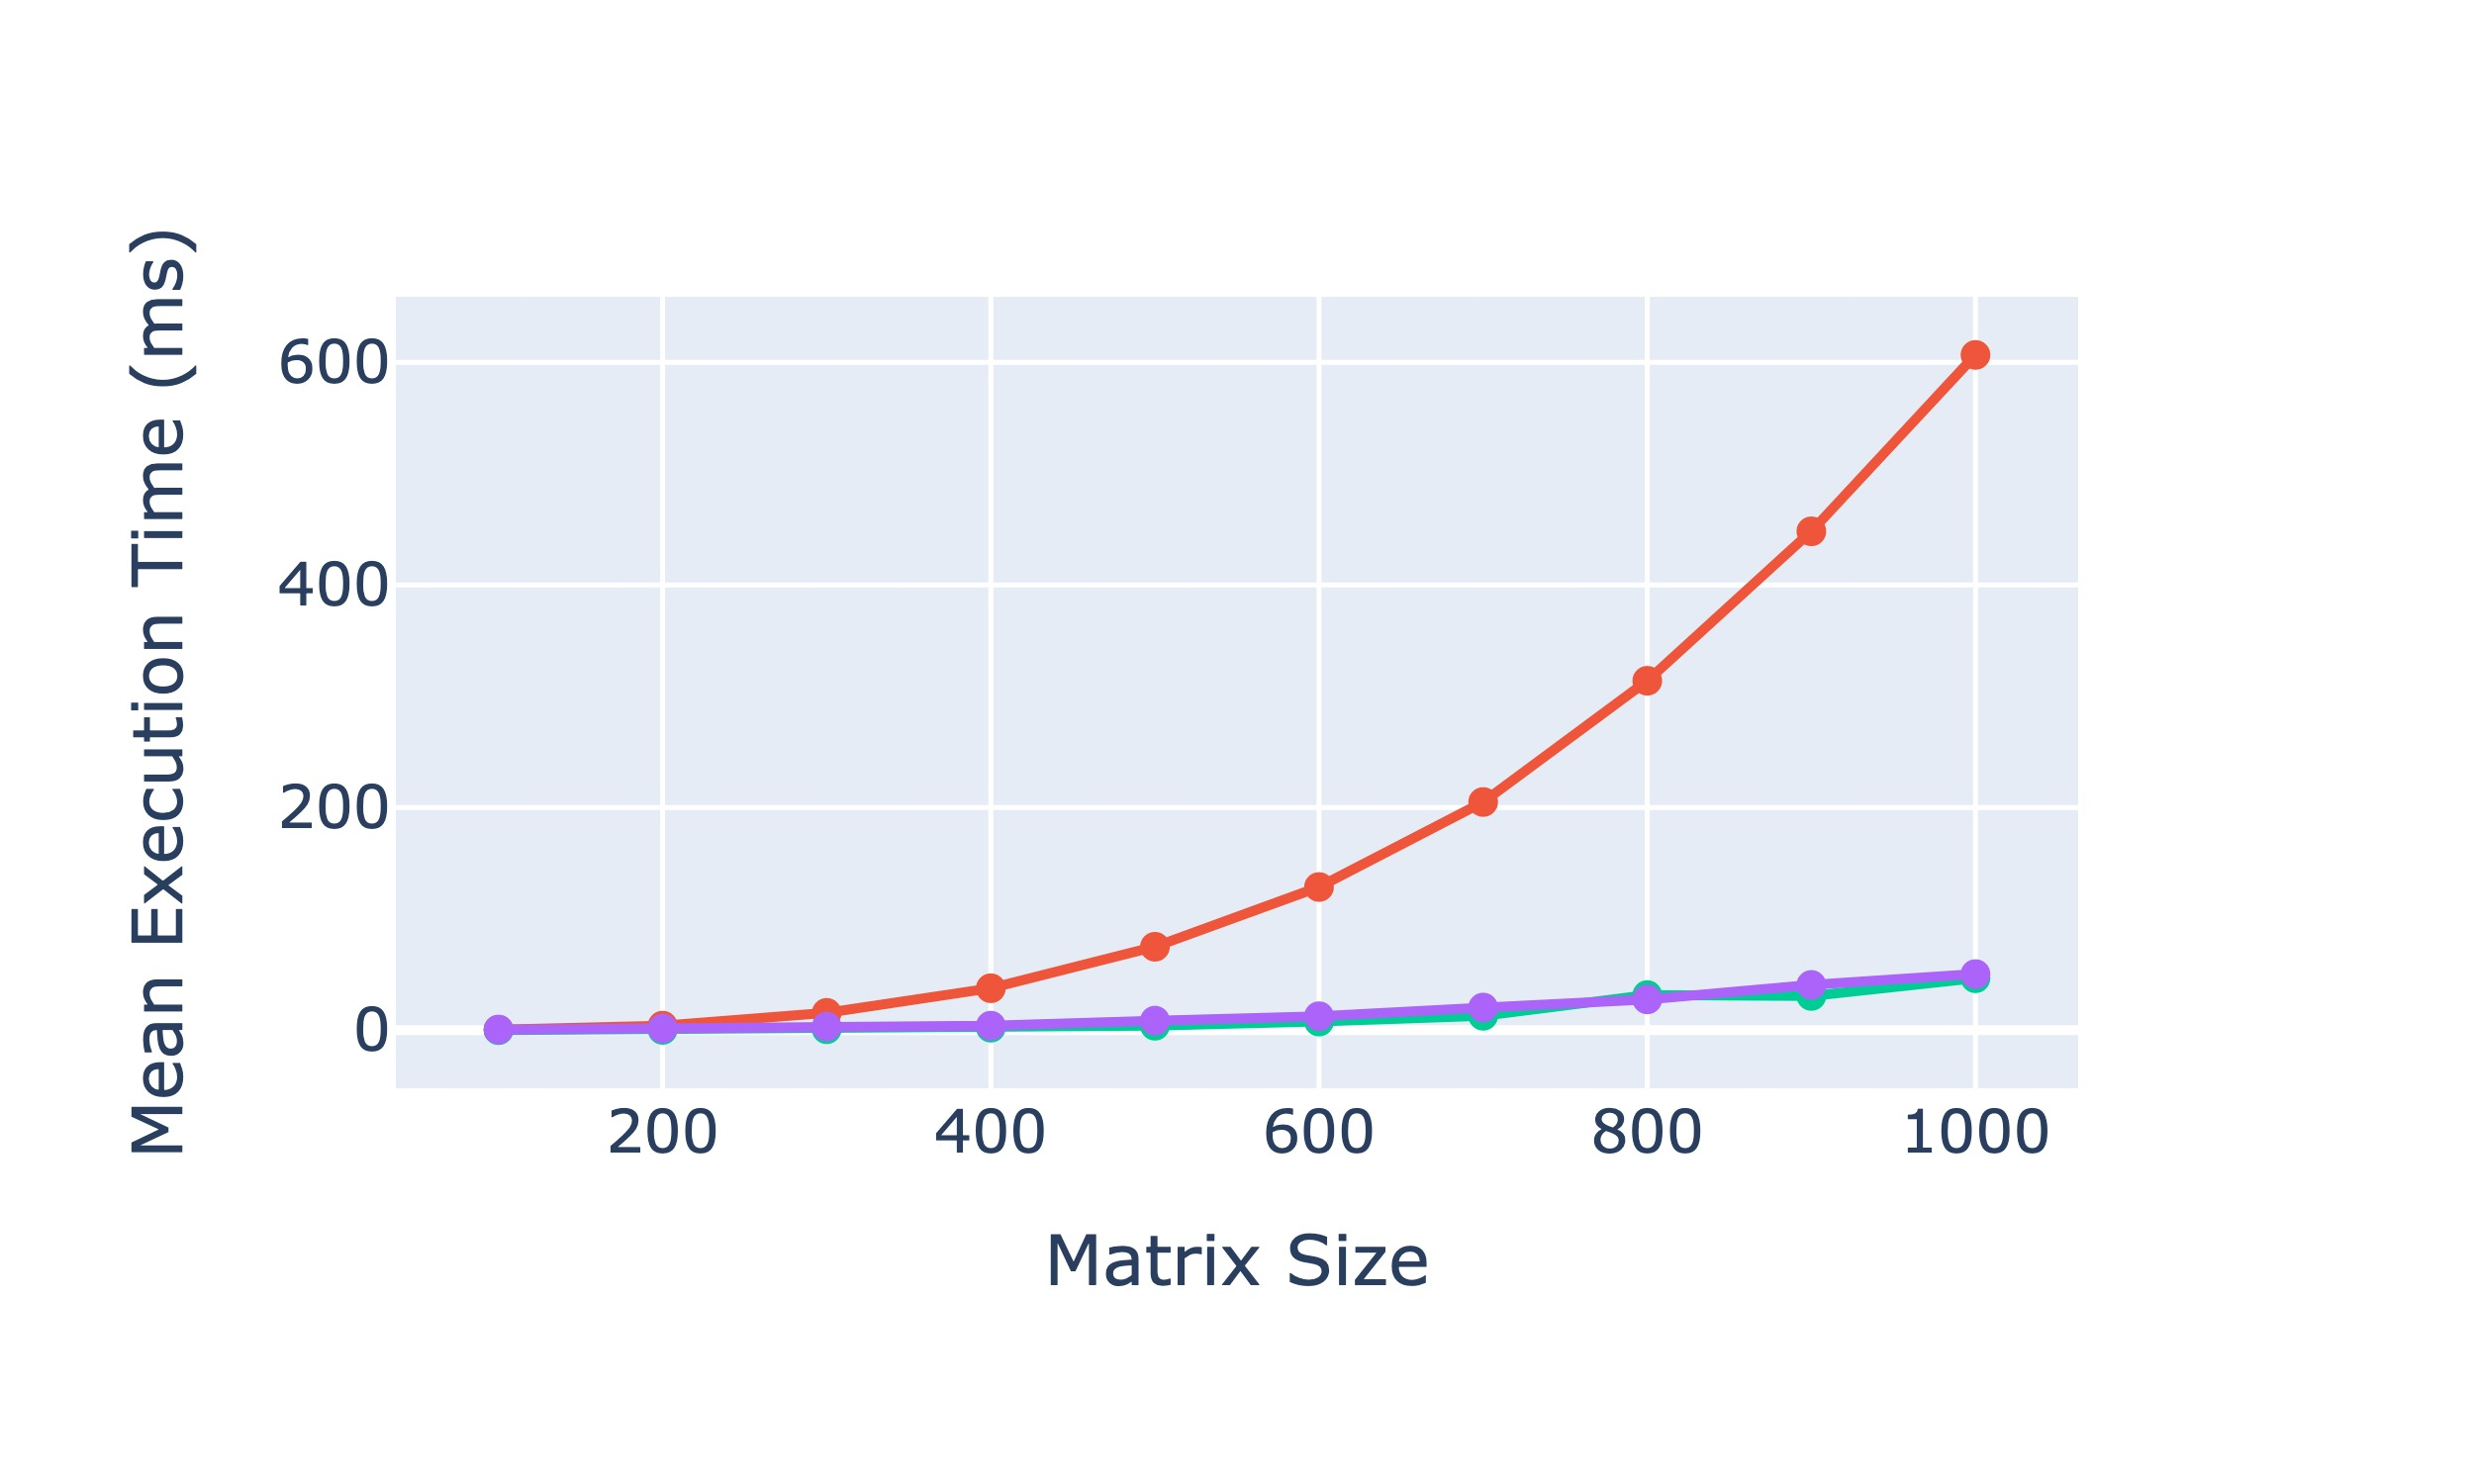
\includegraphics[width=\textwidth]{Images/sparseqr_givens.jpg}
        \caption{Runtime.}
    \end{subfigure}
    % right figure
    \begin{subfigure}[b]{0.48\textwidth}
        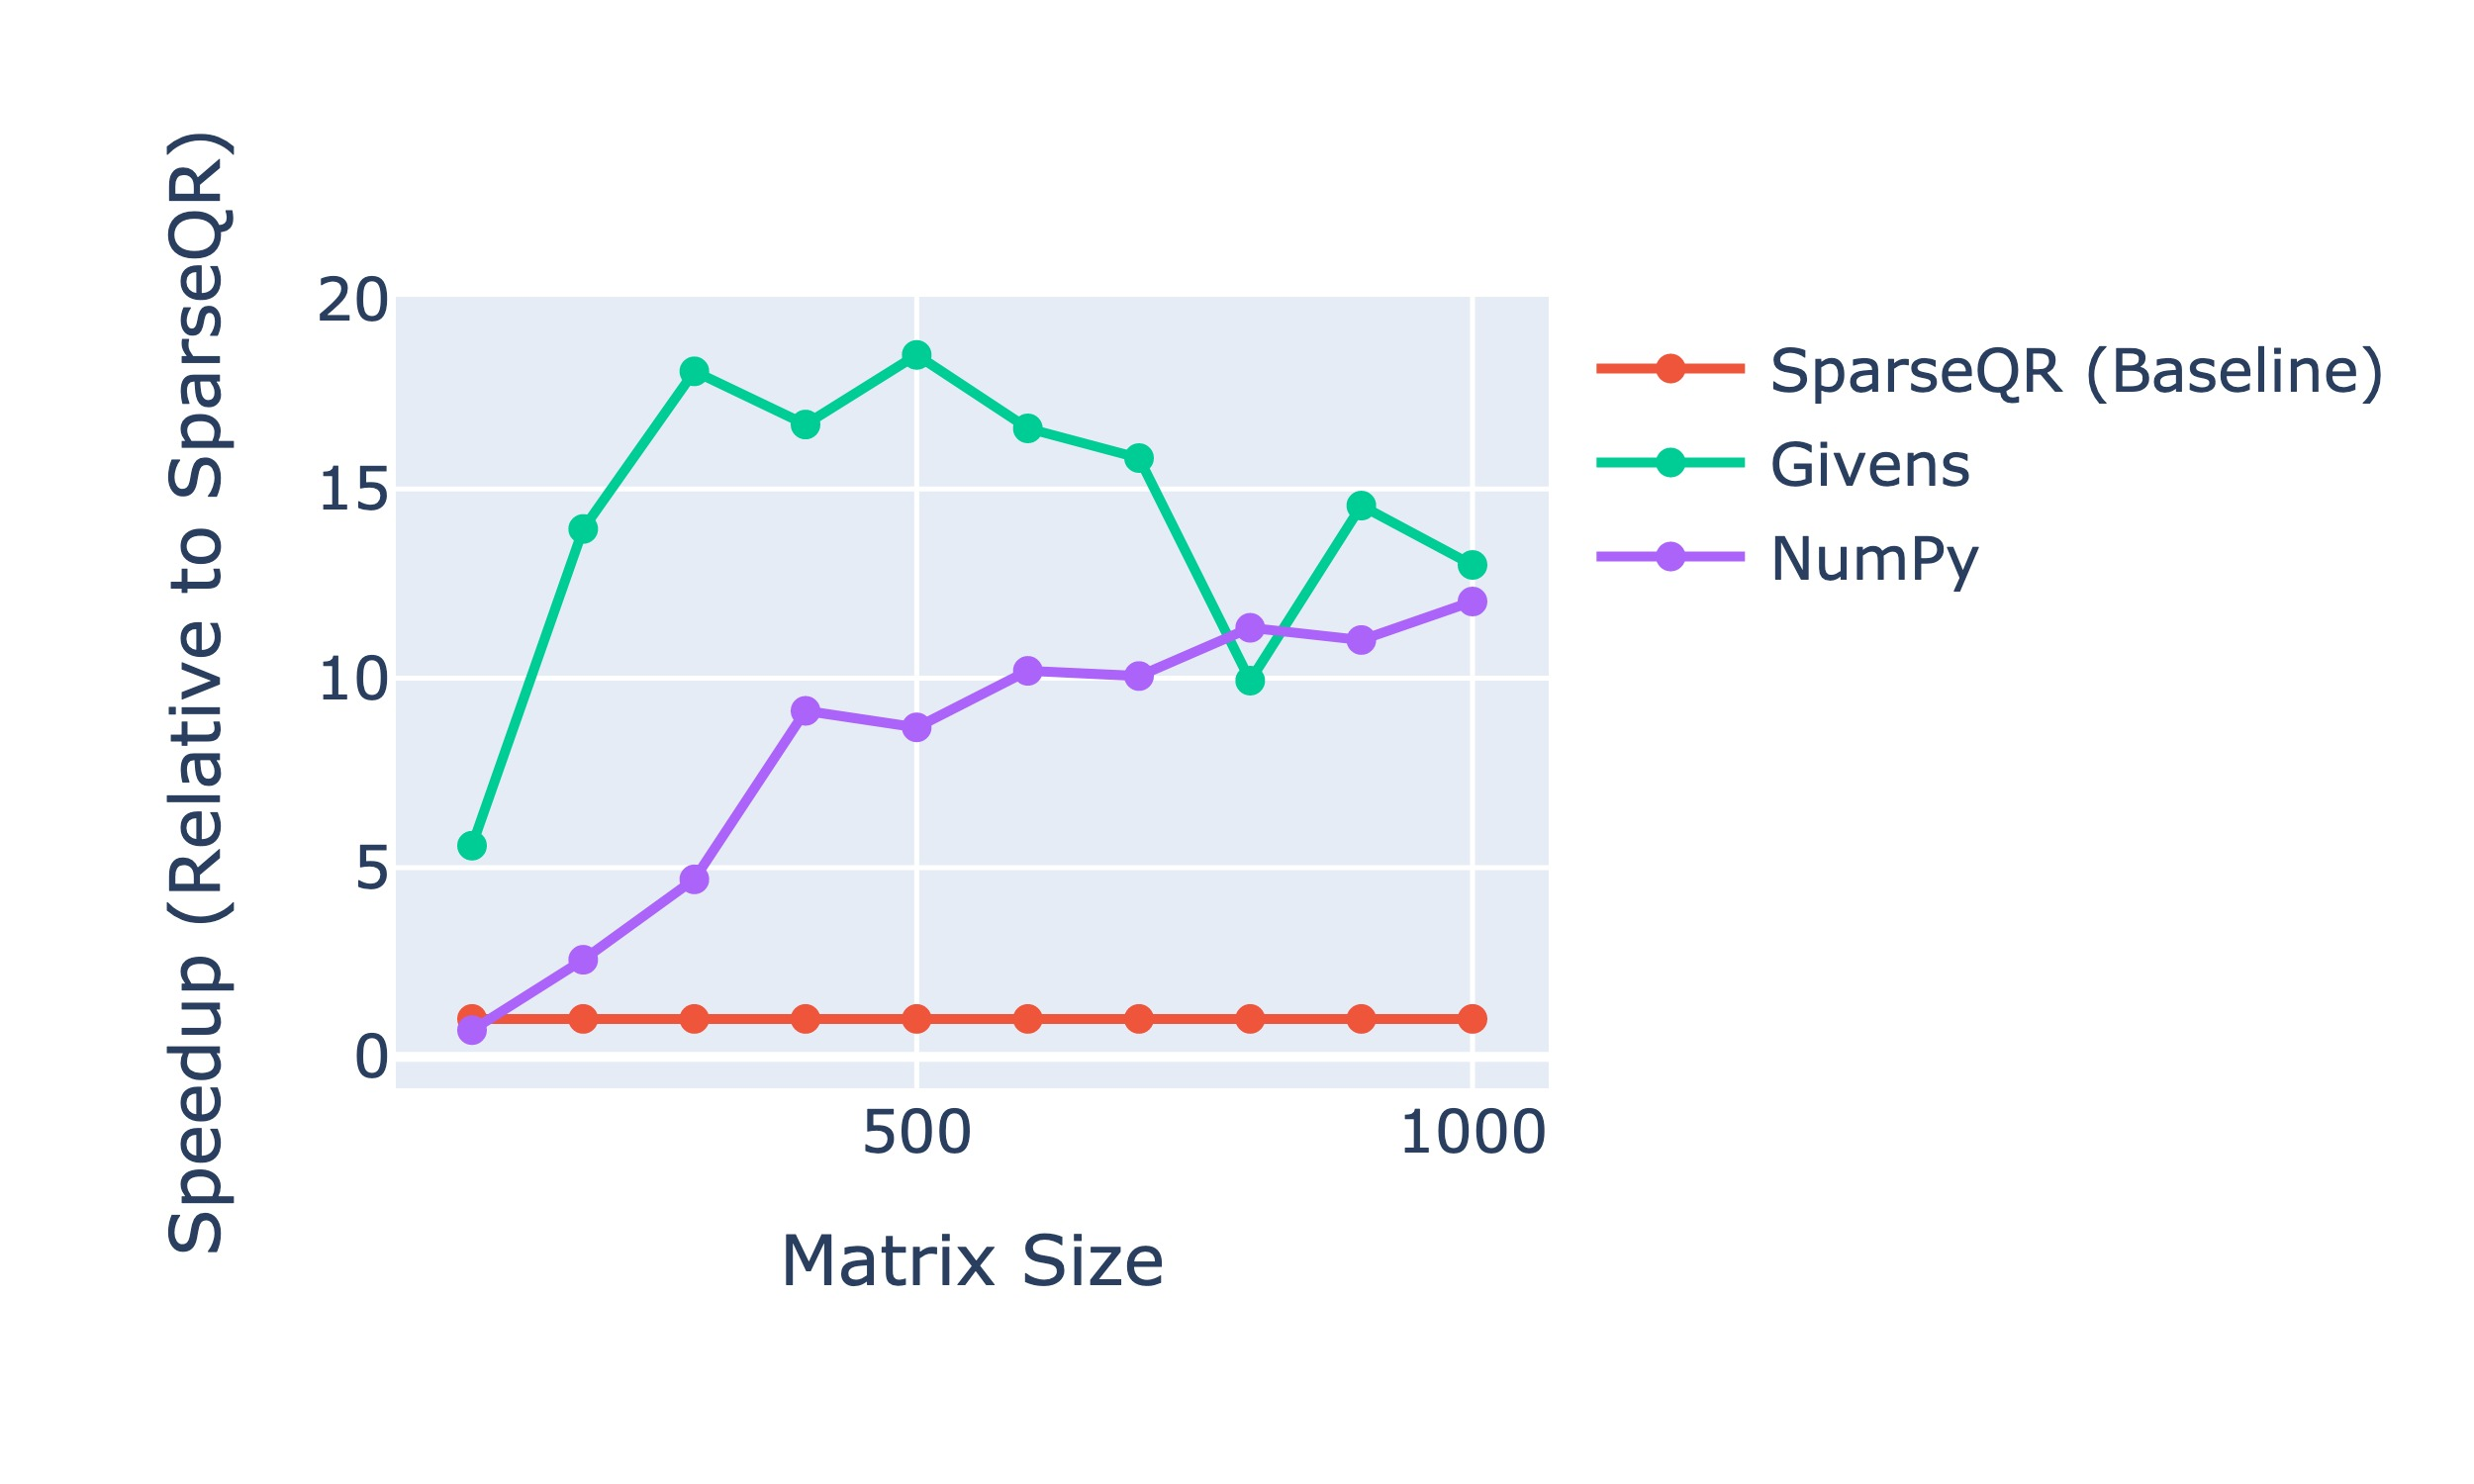
\includegraphics[width=\textwidth]{Images/speedup_sparseqr_givens.jpg}
        \caption{Speedups.}
    \end{subfigure}
    \caption{Computational performance for sparse matrix}
    \label{fig:qr_performance}
\end{figure}

\subsection{Singular Value Decomposition using Power Method}
The singular value decomposition (SVD) is a fundamental matrix decomposition method that decomposes a matrix $A$ into three matrices $U$, $\Sigma$, and $V$ such that:
\[
    A = U \Sigma V^T
\]
where $U$ and $V$ are orthogonal matrices and $\Sigma$ is a diagonal matrix with the singular values of $A$. The SVD is widely used in various applications, including dimensionality reduction, data compression, and machine learning. 

The power method is an iterative algorithm that can be used to compute the singular values and vectors of a matrix. The power method works by repeatedly multiplying the matrix by a vector and normalizing the result. The pseudocode for the power method SVD is shown in Algorithm \ref{alg:power}.

\begin{algorithm}[H]
\caption{Power Method SVD (Rank-$k$ Approximation)}
\begin{algorithmic}[1]
\label{alg:power}
\REQUIRE Matrix $A \in \mathbb{R}^{m \times n}$, target rank $k$, tolerance $\epsilon_\delta$, factor $\delta$, and parameter $\lambda$
\ENSURE Approximate singular values $\sigma_i$ and singular vectors $u_i, v_i$ for $i = 1 \dots k$
\FOR{$i = 1$ \textbf{to} $k$}
  \STATE $s \gets log(4log(2n / \sigma / \epsilon \sigma) / 2 \lambda$


  \STATE $v \gets \text{RandomNormal}(n)$ 

  \FOR{$\ell = 1$ \textbf{to} $s$}
    \STATE $v \gets A^\top (A v)$
    \STATE $v \gets v / \|v\|$
  \ENDFOR

  \STATE $\sigma \gets \|A\,v\|$
  \STATE $u \gets (A\,v)/\sigma$

  \IF{$\sigma < 10^{-14}$}
    \STATE \textbf{break}
  \ENDIF

  \STATE $\sigma_i \gets \sigma,\; u_i \gets u,\; v_i \gets v$
  \STATE $A \gets A - \sigma \,u\, v^\top$
\ENDFOR

\end{algorithmic}
\end{algorithm}


\subsection{RSVD Implementation}
Let $A \in \mathbb{R}^{m \times n}$ be a matrix of low rank, and $m \ge n$. 
In the following, we seek the near-optimal low-rank approximation of the form
\[
A \approx U_k \Sigma_k V_k^T
\]
where $k$ denotes the target rank. Instead of computing the singular value decomposition directly, we embed the SVD into the probabilistic framework. The principal concept is sketched in Figure \ref{fig:rSVD}.

We implemented the RSVD algorithm using \texttt{Eigen} library, the QR decomposition, and svd algorithm mentioned above. We defined the following explicit template instantiation and specialization:
\begin{minted}[fontsize=\small, linenos, frame=single]{cpp}
// Dense matrix
Eigen::RandomizedSVD<double, Eigen::Dynamic, Eigen::Dynamic> rsvd;
// Sparse matrix
Eigen::RandomizedSVD<Eigen::SparseMatrix<double>>
// Row-major matrix
Eigen::RandomizedSVD<Eigen::SparseMatrix<double, Eigen::RowMajor>>
\end{minted}

\begin{figure}[H]
    \centering
    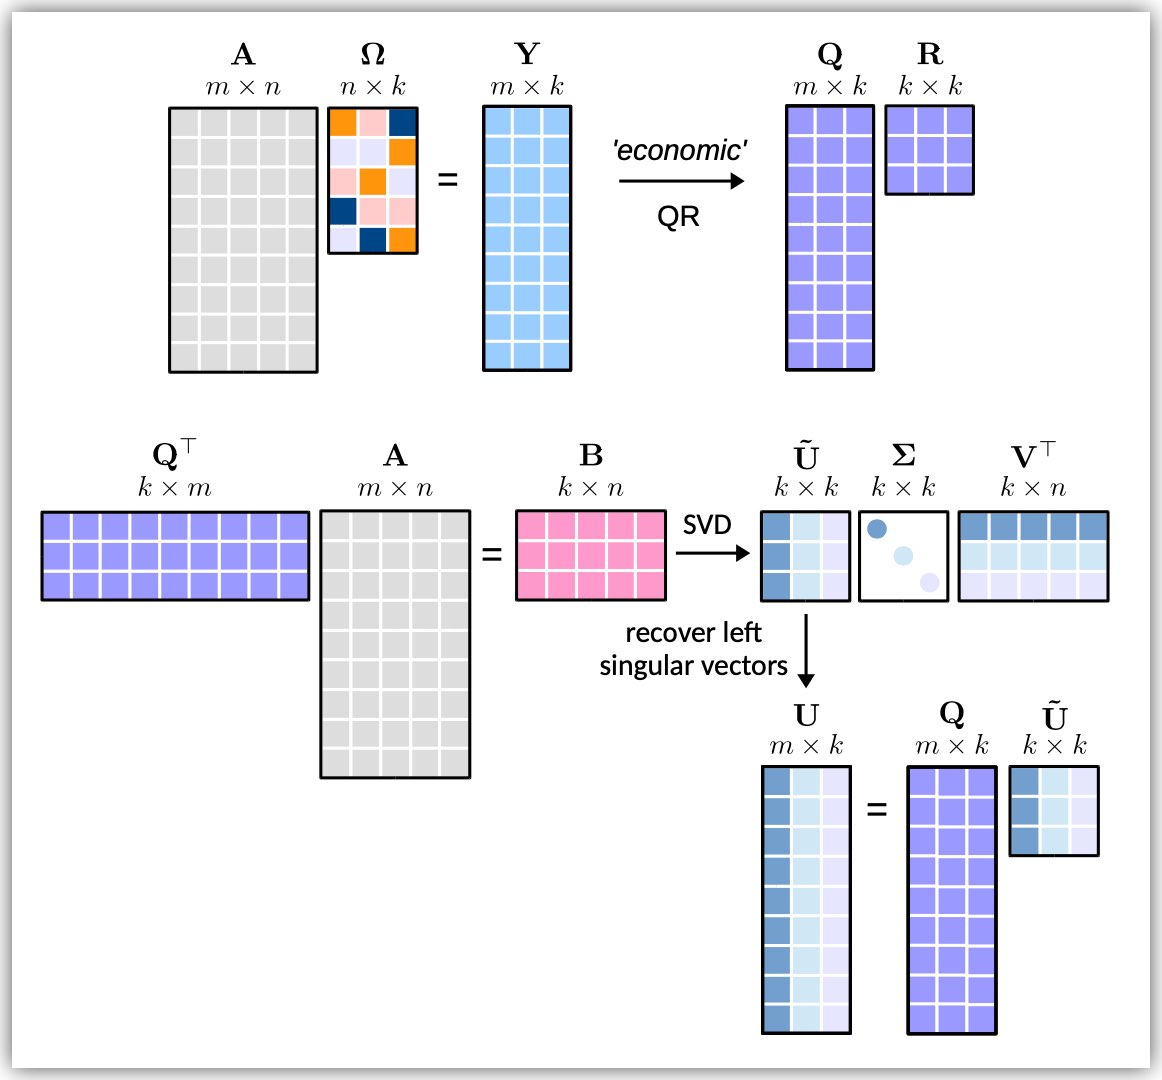
\includegraphics[height=0.2\textheight]{Images/rSVD.jpg}
    \caption{Randomized SVD \cite{erichsonRandomizedMatrixDecompositions2019}}
    \label{fig:rSVD}
\end{figure}

We now investigate the performance of the implementation in more detail. Figures \ref{fig:dense_rsvd} shows the performance of varying target ranks. The speedups show the relative performance compared to the base \texttt{BDCSVD} in \texttt{Eigen}. The relative reconstruction error is computed as \[ \frac{\|\mathbf{A} - \mathbf{A}_k\|_F}{\|\mathbf{A}\|_F} \] The implementation of rsvd achieves substantial speedups over the other implementation of SVD. Obviously, increasing the number of power iteration can improve accuracy, we can control the trade-off between computational time and accuracy, depending on the application. Regarding errors, all methods can converge to \textbf{1e-15}, with \texttt{PowerSVD} being more accurate.

\begin{figure}[htbp]
    \centering
    % First plot
    \begin{subfigure}[b]{0.31\textwidth}
        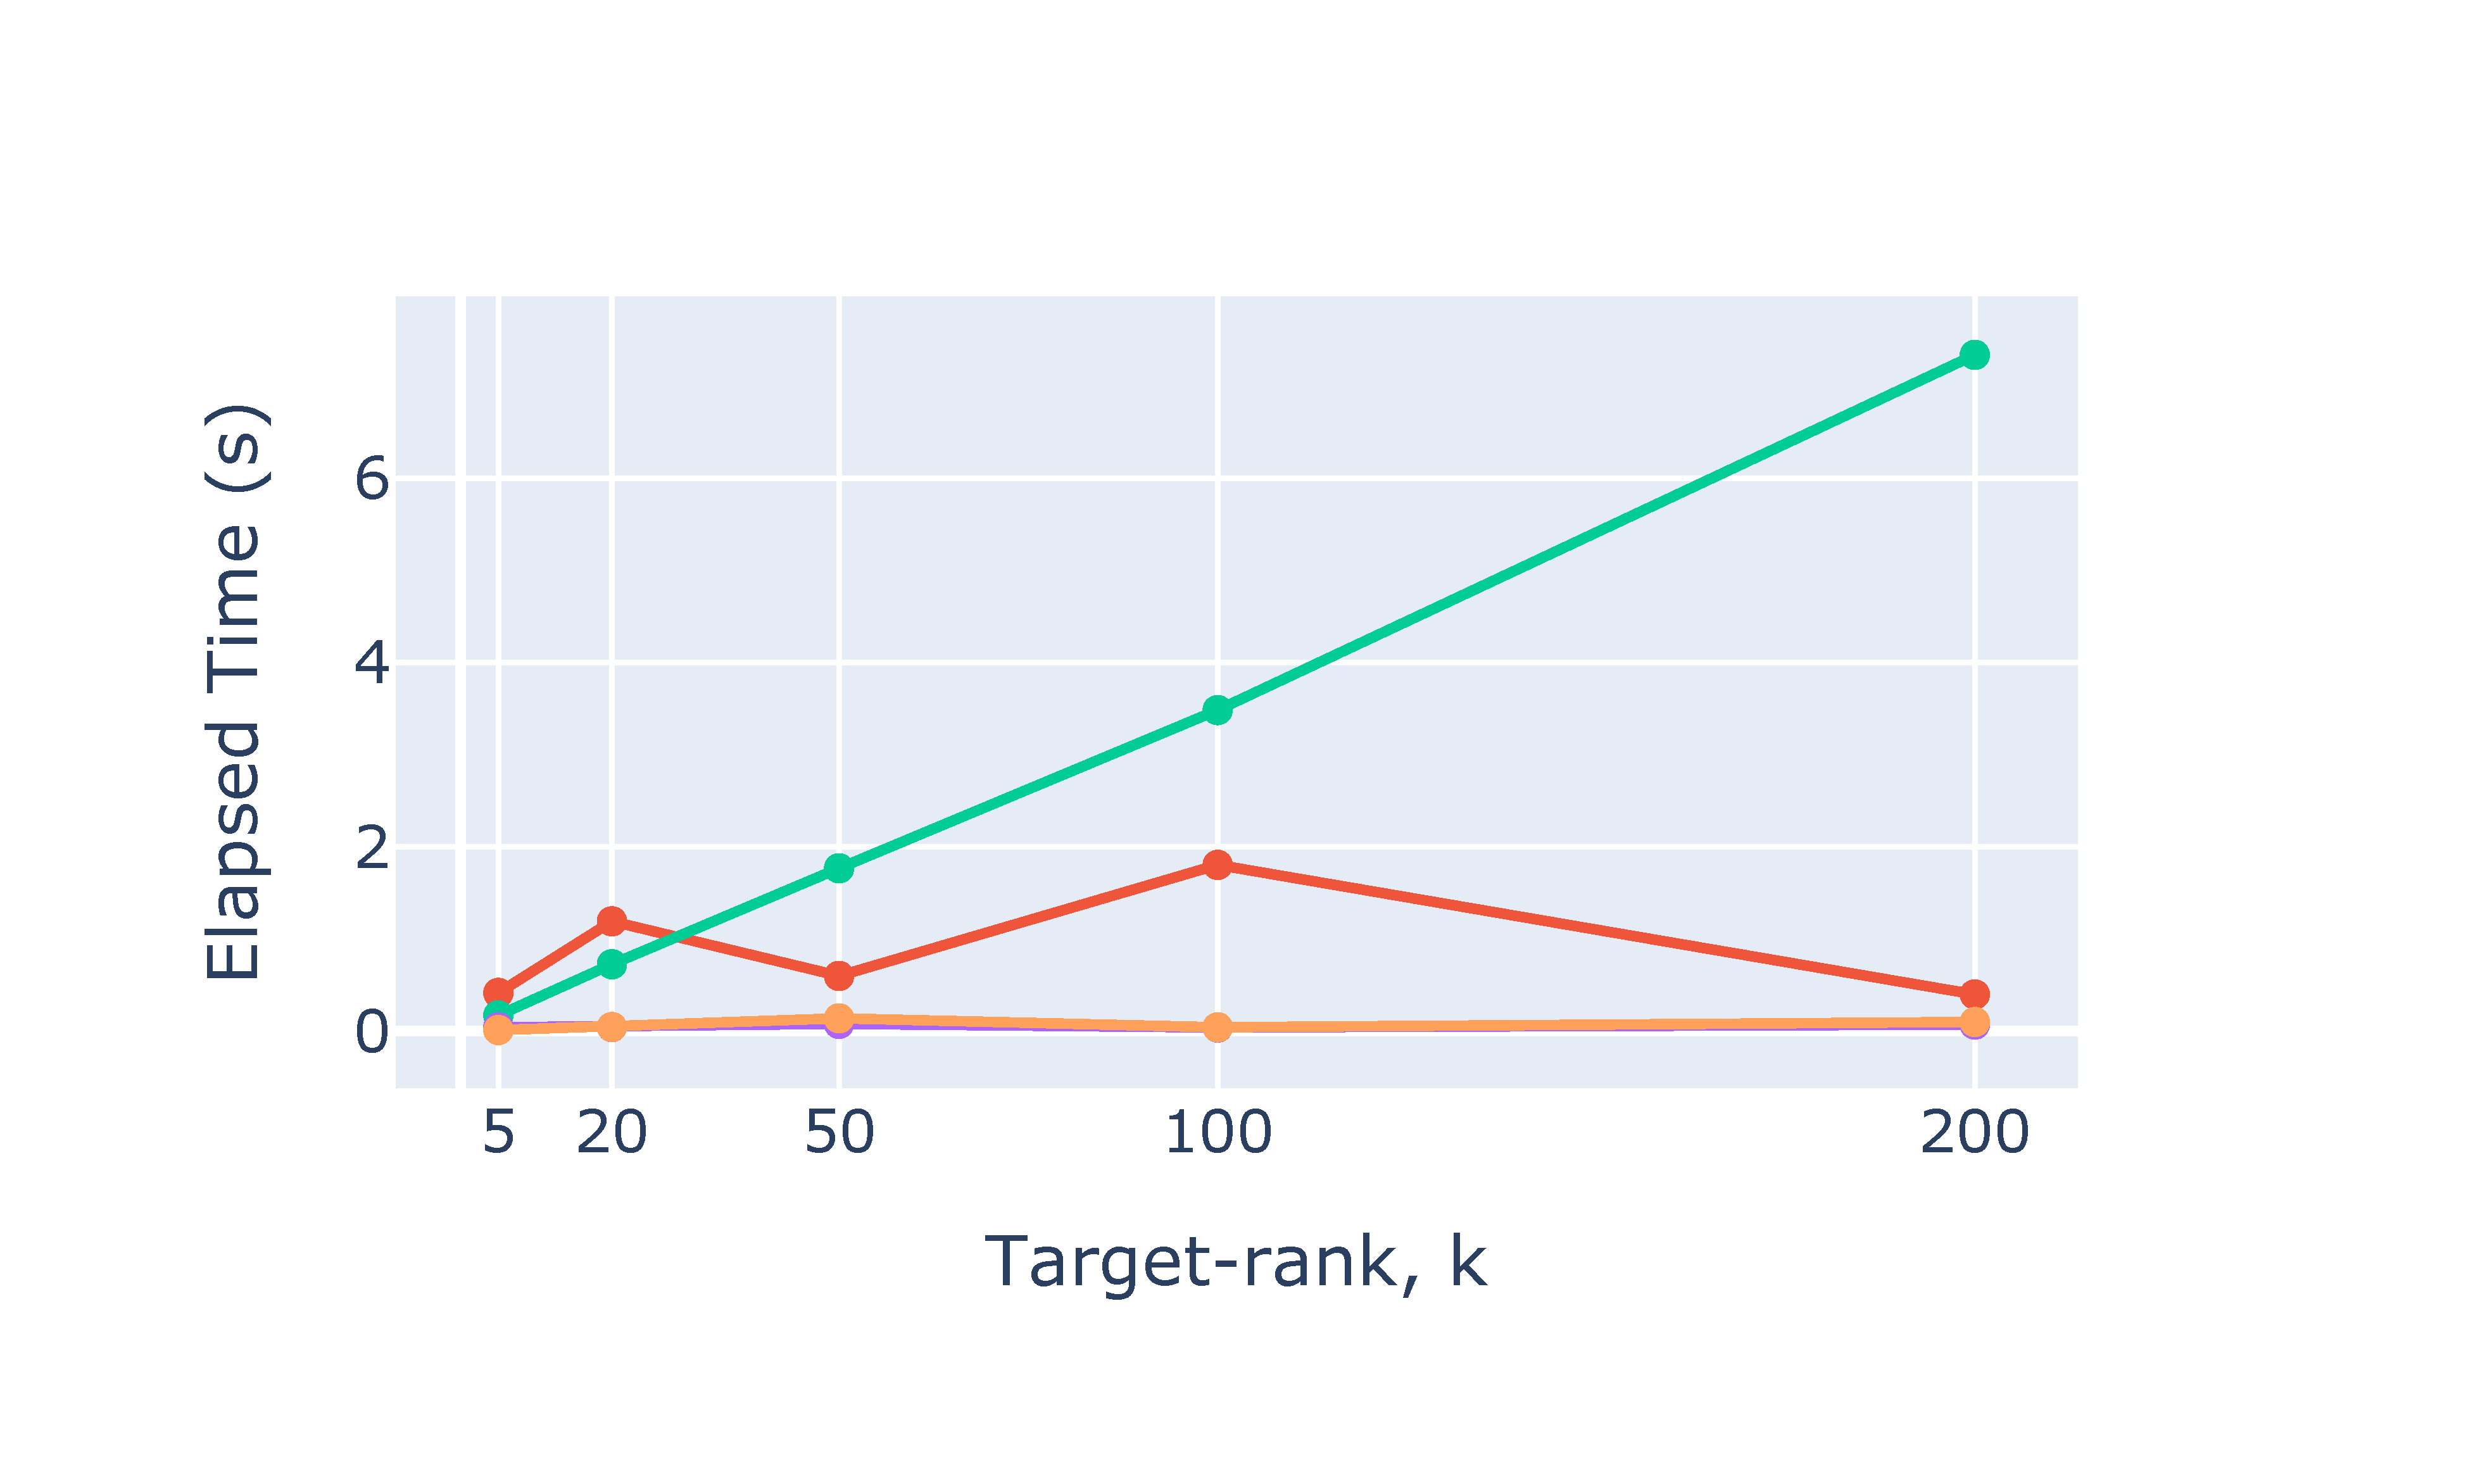
\includegraphics[width=\textwidth, trim={100 100 100 100}, clip]{Images/svd_time.pdf}
        \caption{Runtime.}
        \label{fig:runtime}
    \end{subfigure}
    \hfill
    % Second plot
    \begin{subfigure}[b]{0.31\textwidth}
        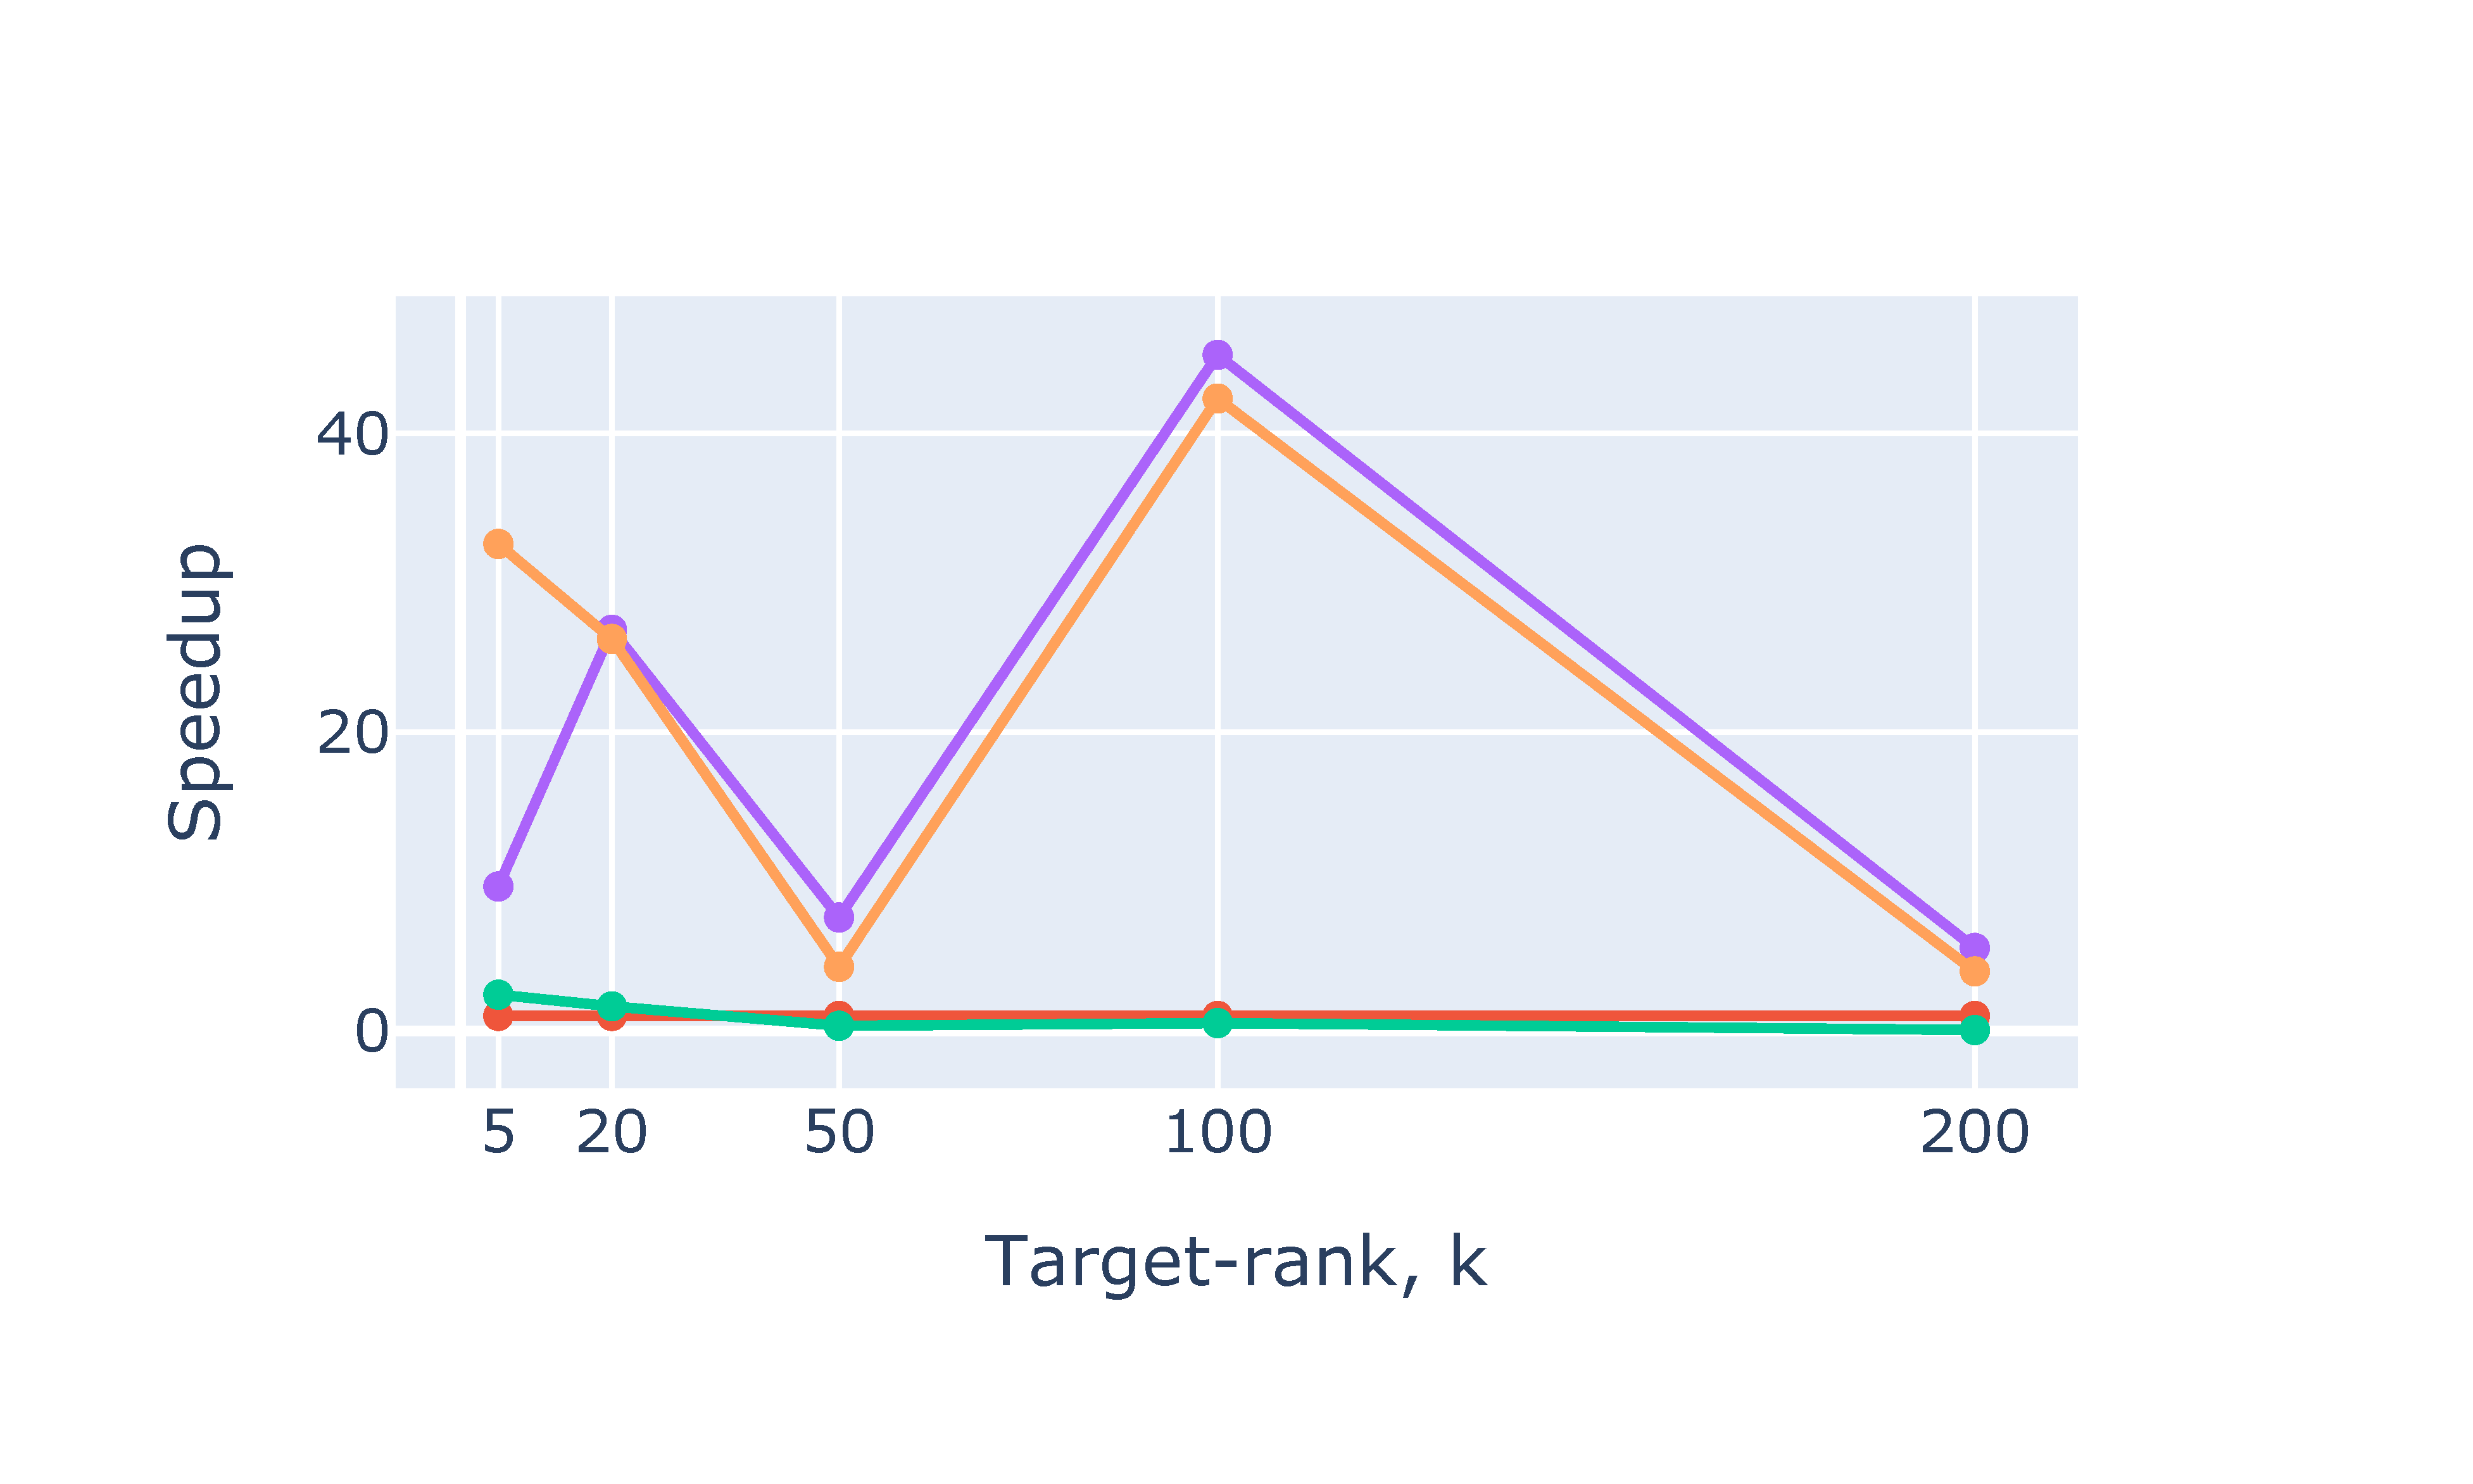
\includegraphics[width=\textwidth, trim={100 100 100 100}, clip]{Images/svd_speedup.pdf}
        \caption{Speedups.}
        \label{fig:speedups}
    \end{subfigure}
    \hfill
    % Third plot
    \begin{subfigure}[b]{0.31\textwidth}
        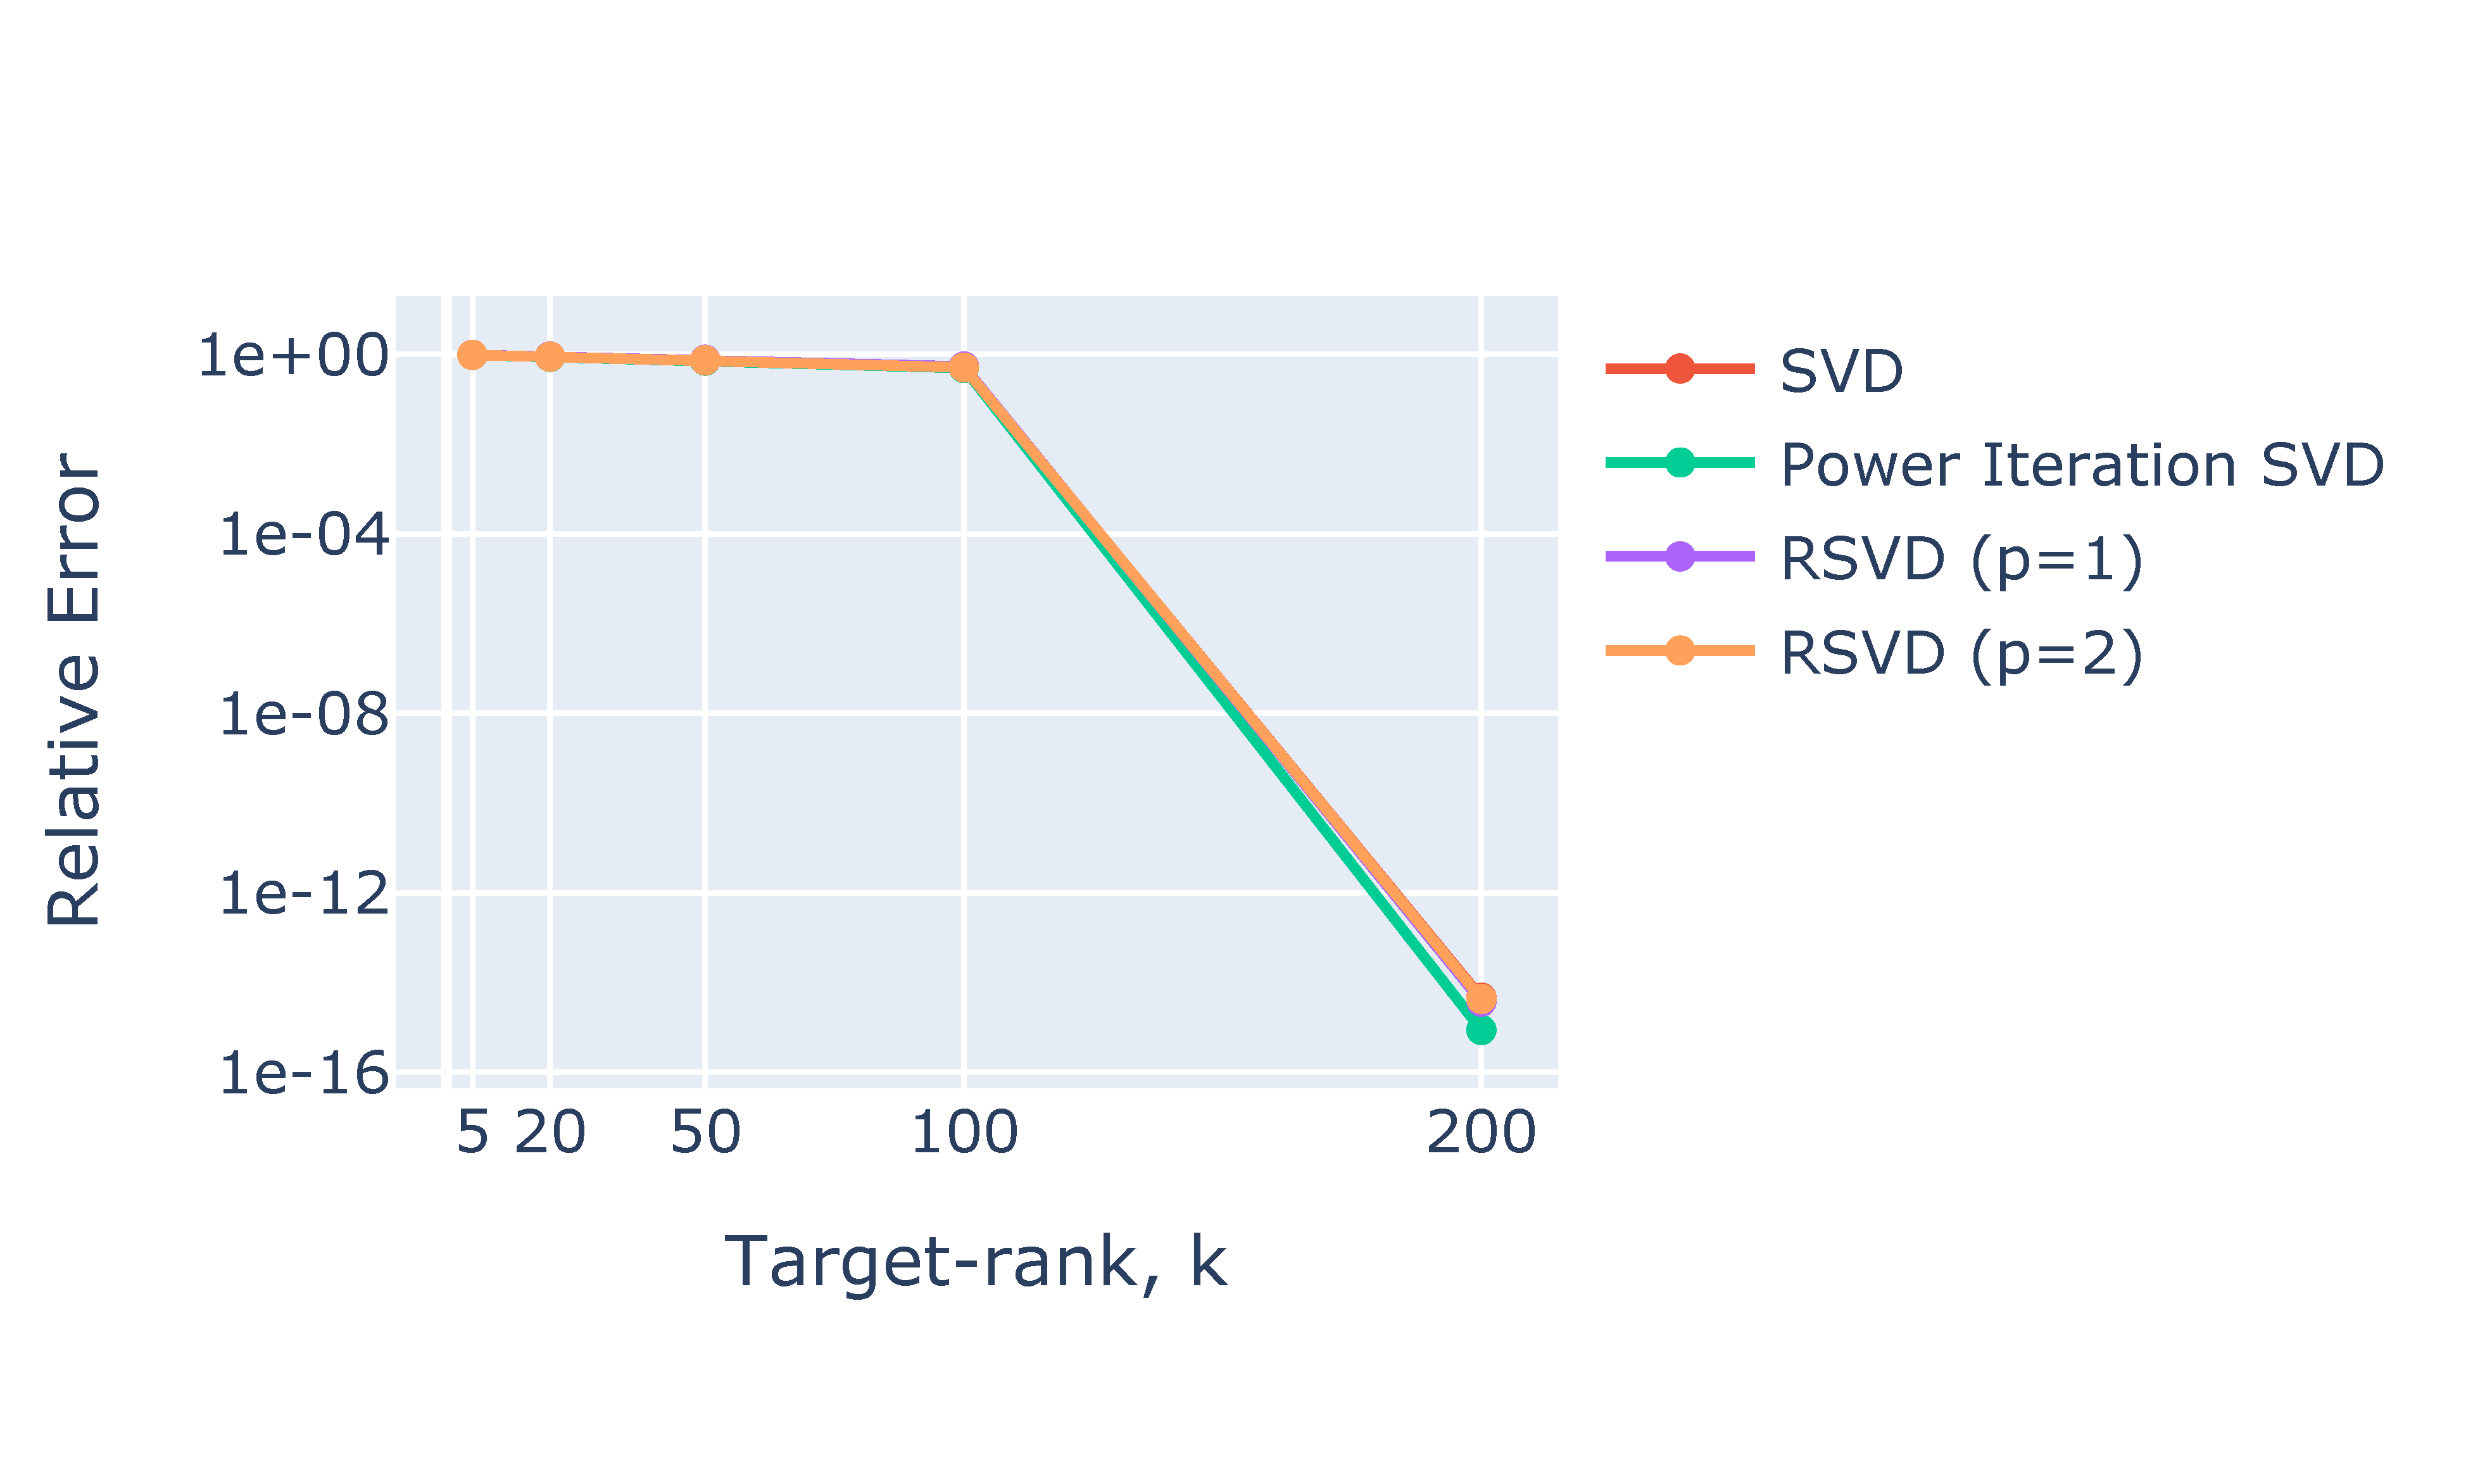
\includegraphics[width=\textwidth, trim={100 100 100 100}, clip]{Images/svd_error.pdf}
        \caption{Relative errors.}
        \label{fig:errors}
    \end{subfigure}

    \caption{Computational performance for a dense $1000 \times 1000$ matrix}
    \label{fig:dense_rsvd}
\end{figure}

\begin{figure}[htbp]
    \centering
    % First plot
    \begin{subfigure}[b]{0.31\textwidth}
        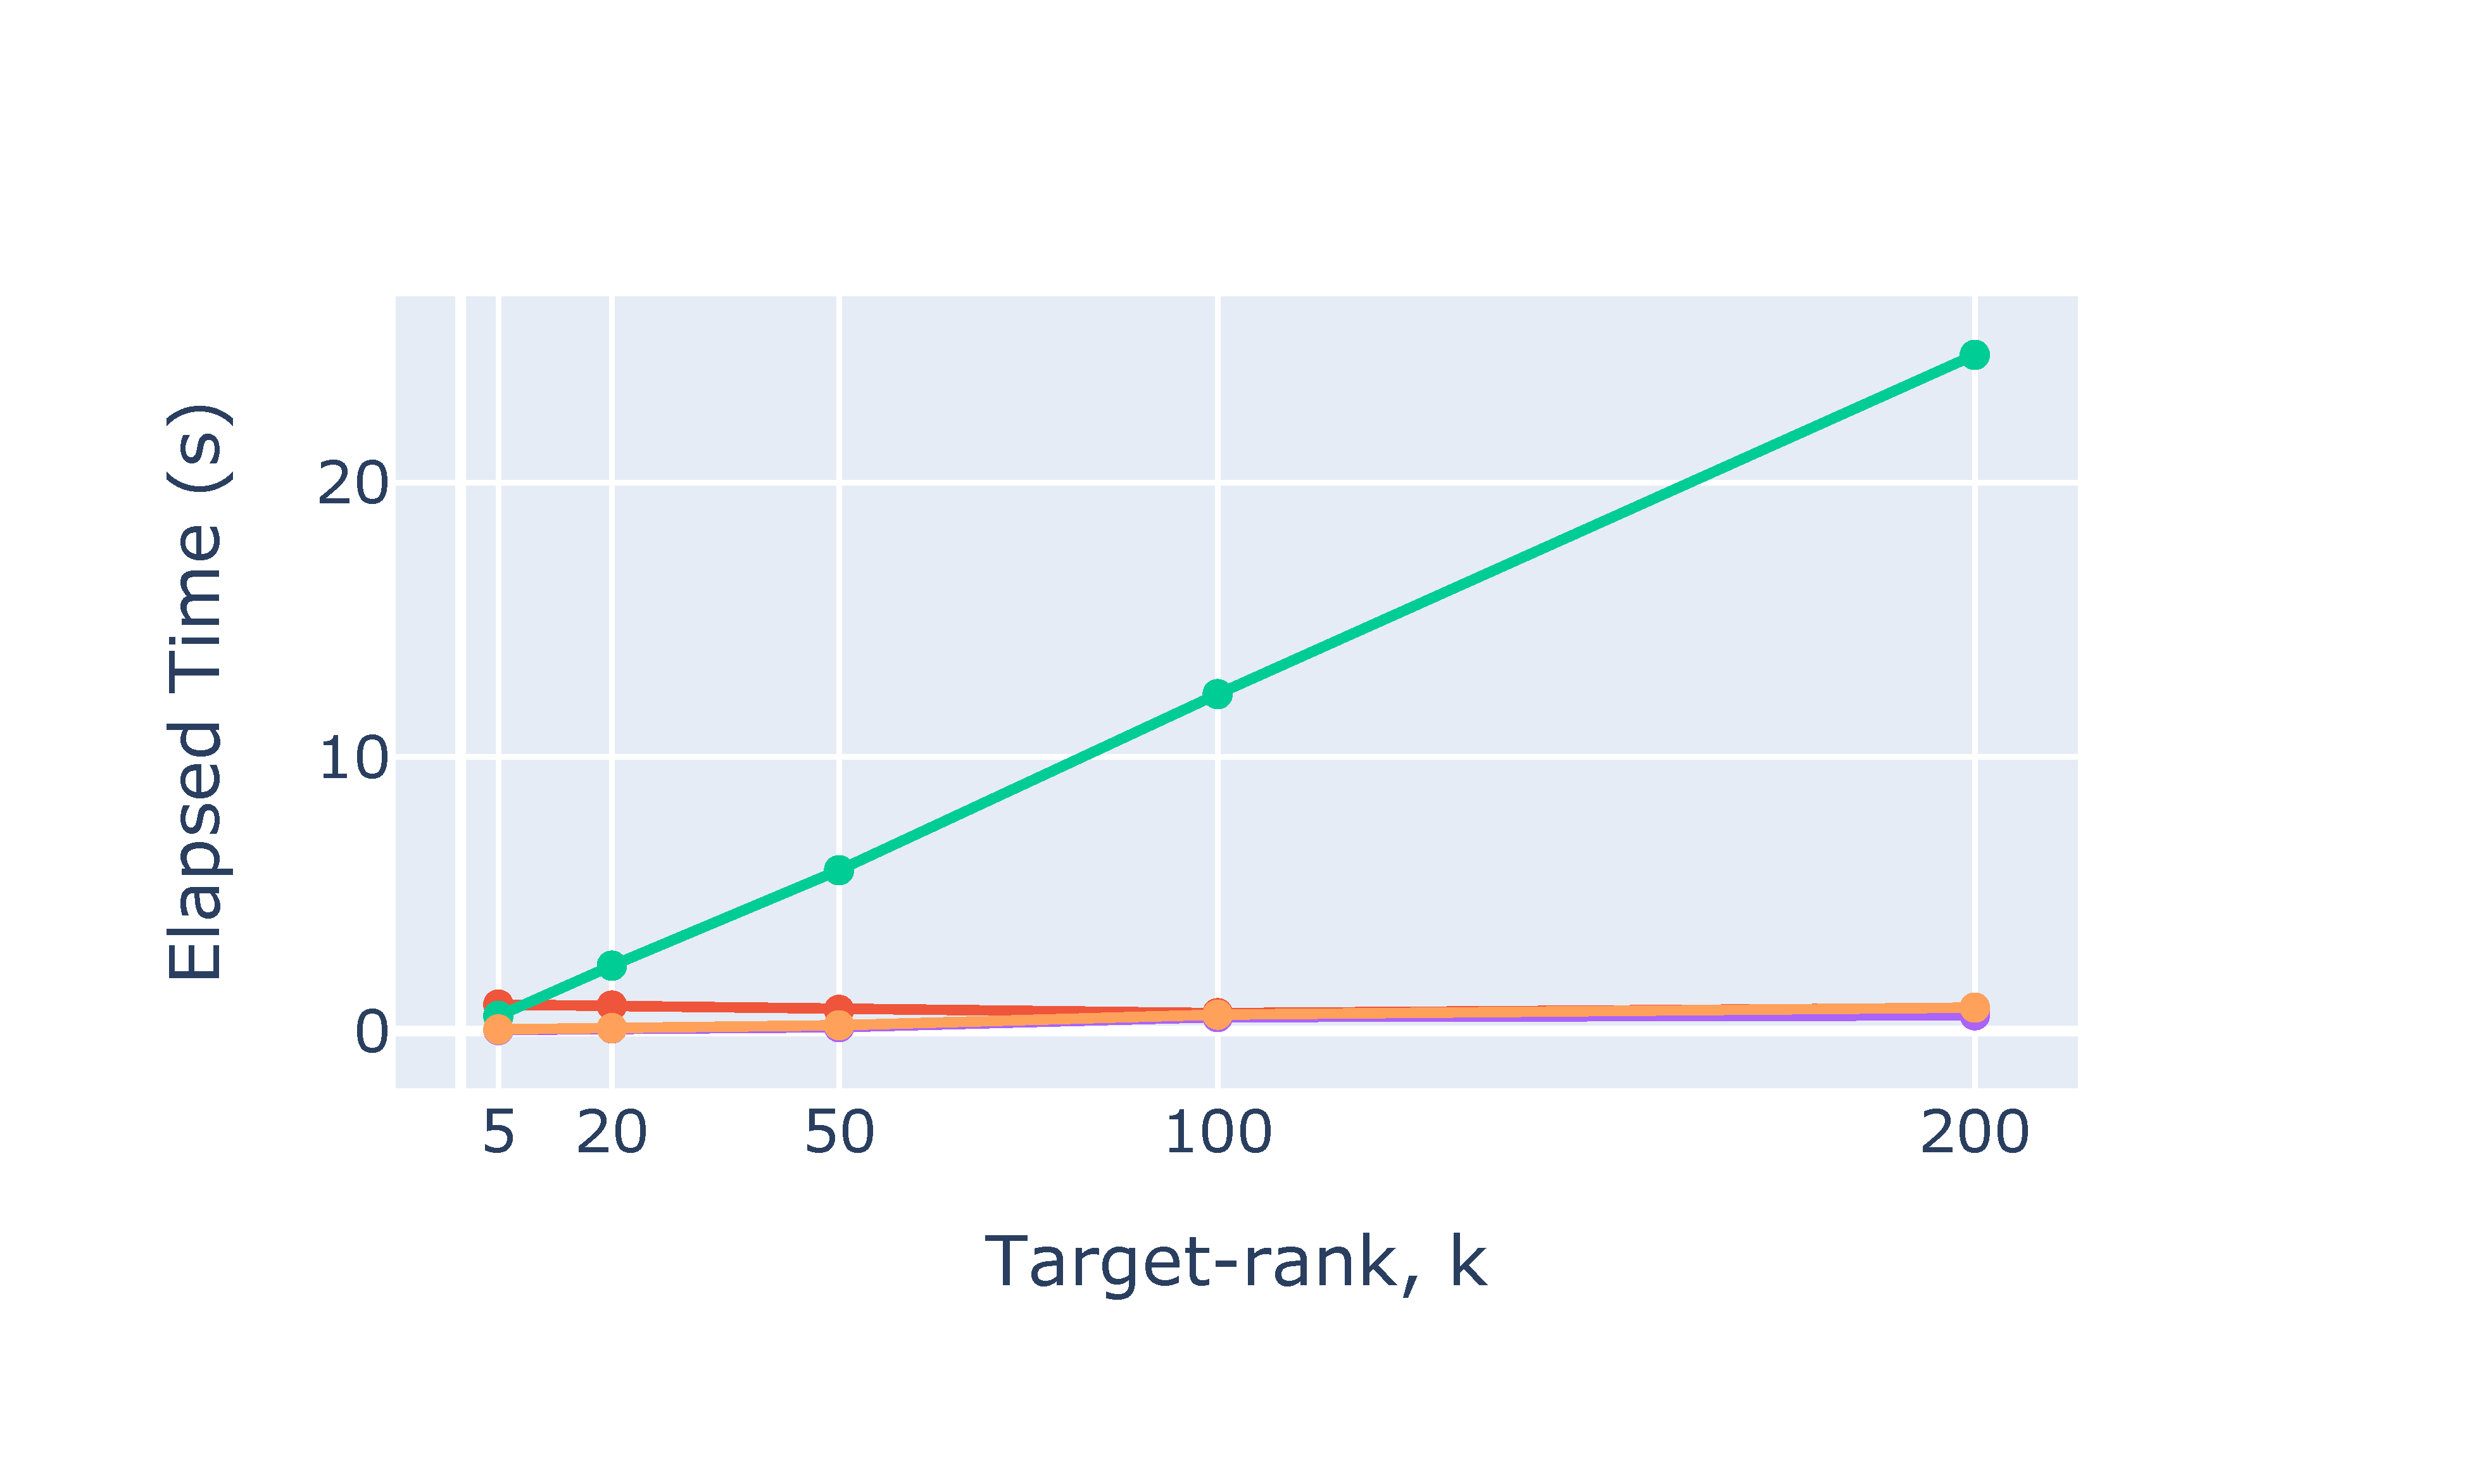
\includegraphics[width=\textwidth, trim={100 100 100 100}, clip]{Images/svd_time_sparse.pdf}
        \caption{Runtime.}
        \label{fig:runtime}
    \end{subfigure}
    \hfill
    % Second plot
    \begin{subfigure}[b]{0.31\textwidth}
        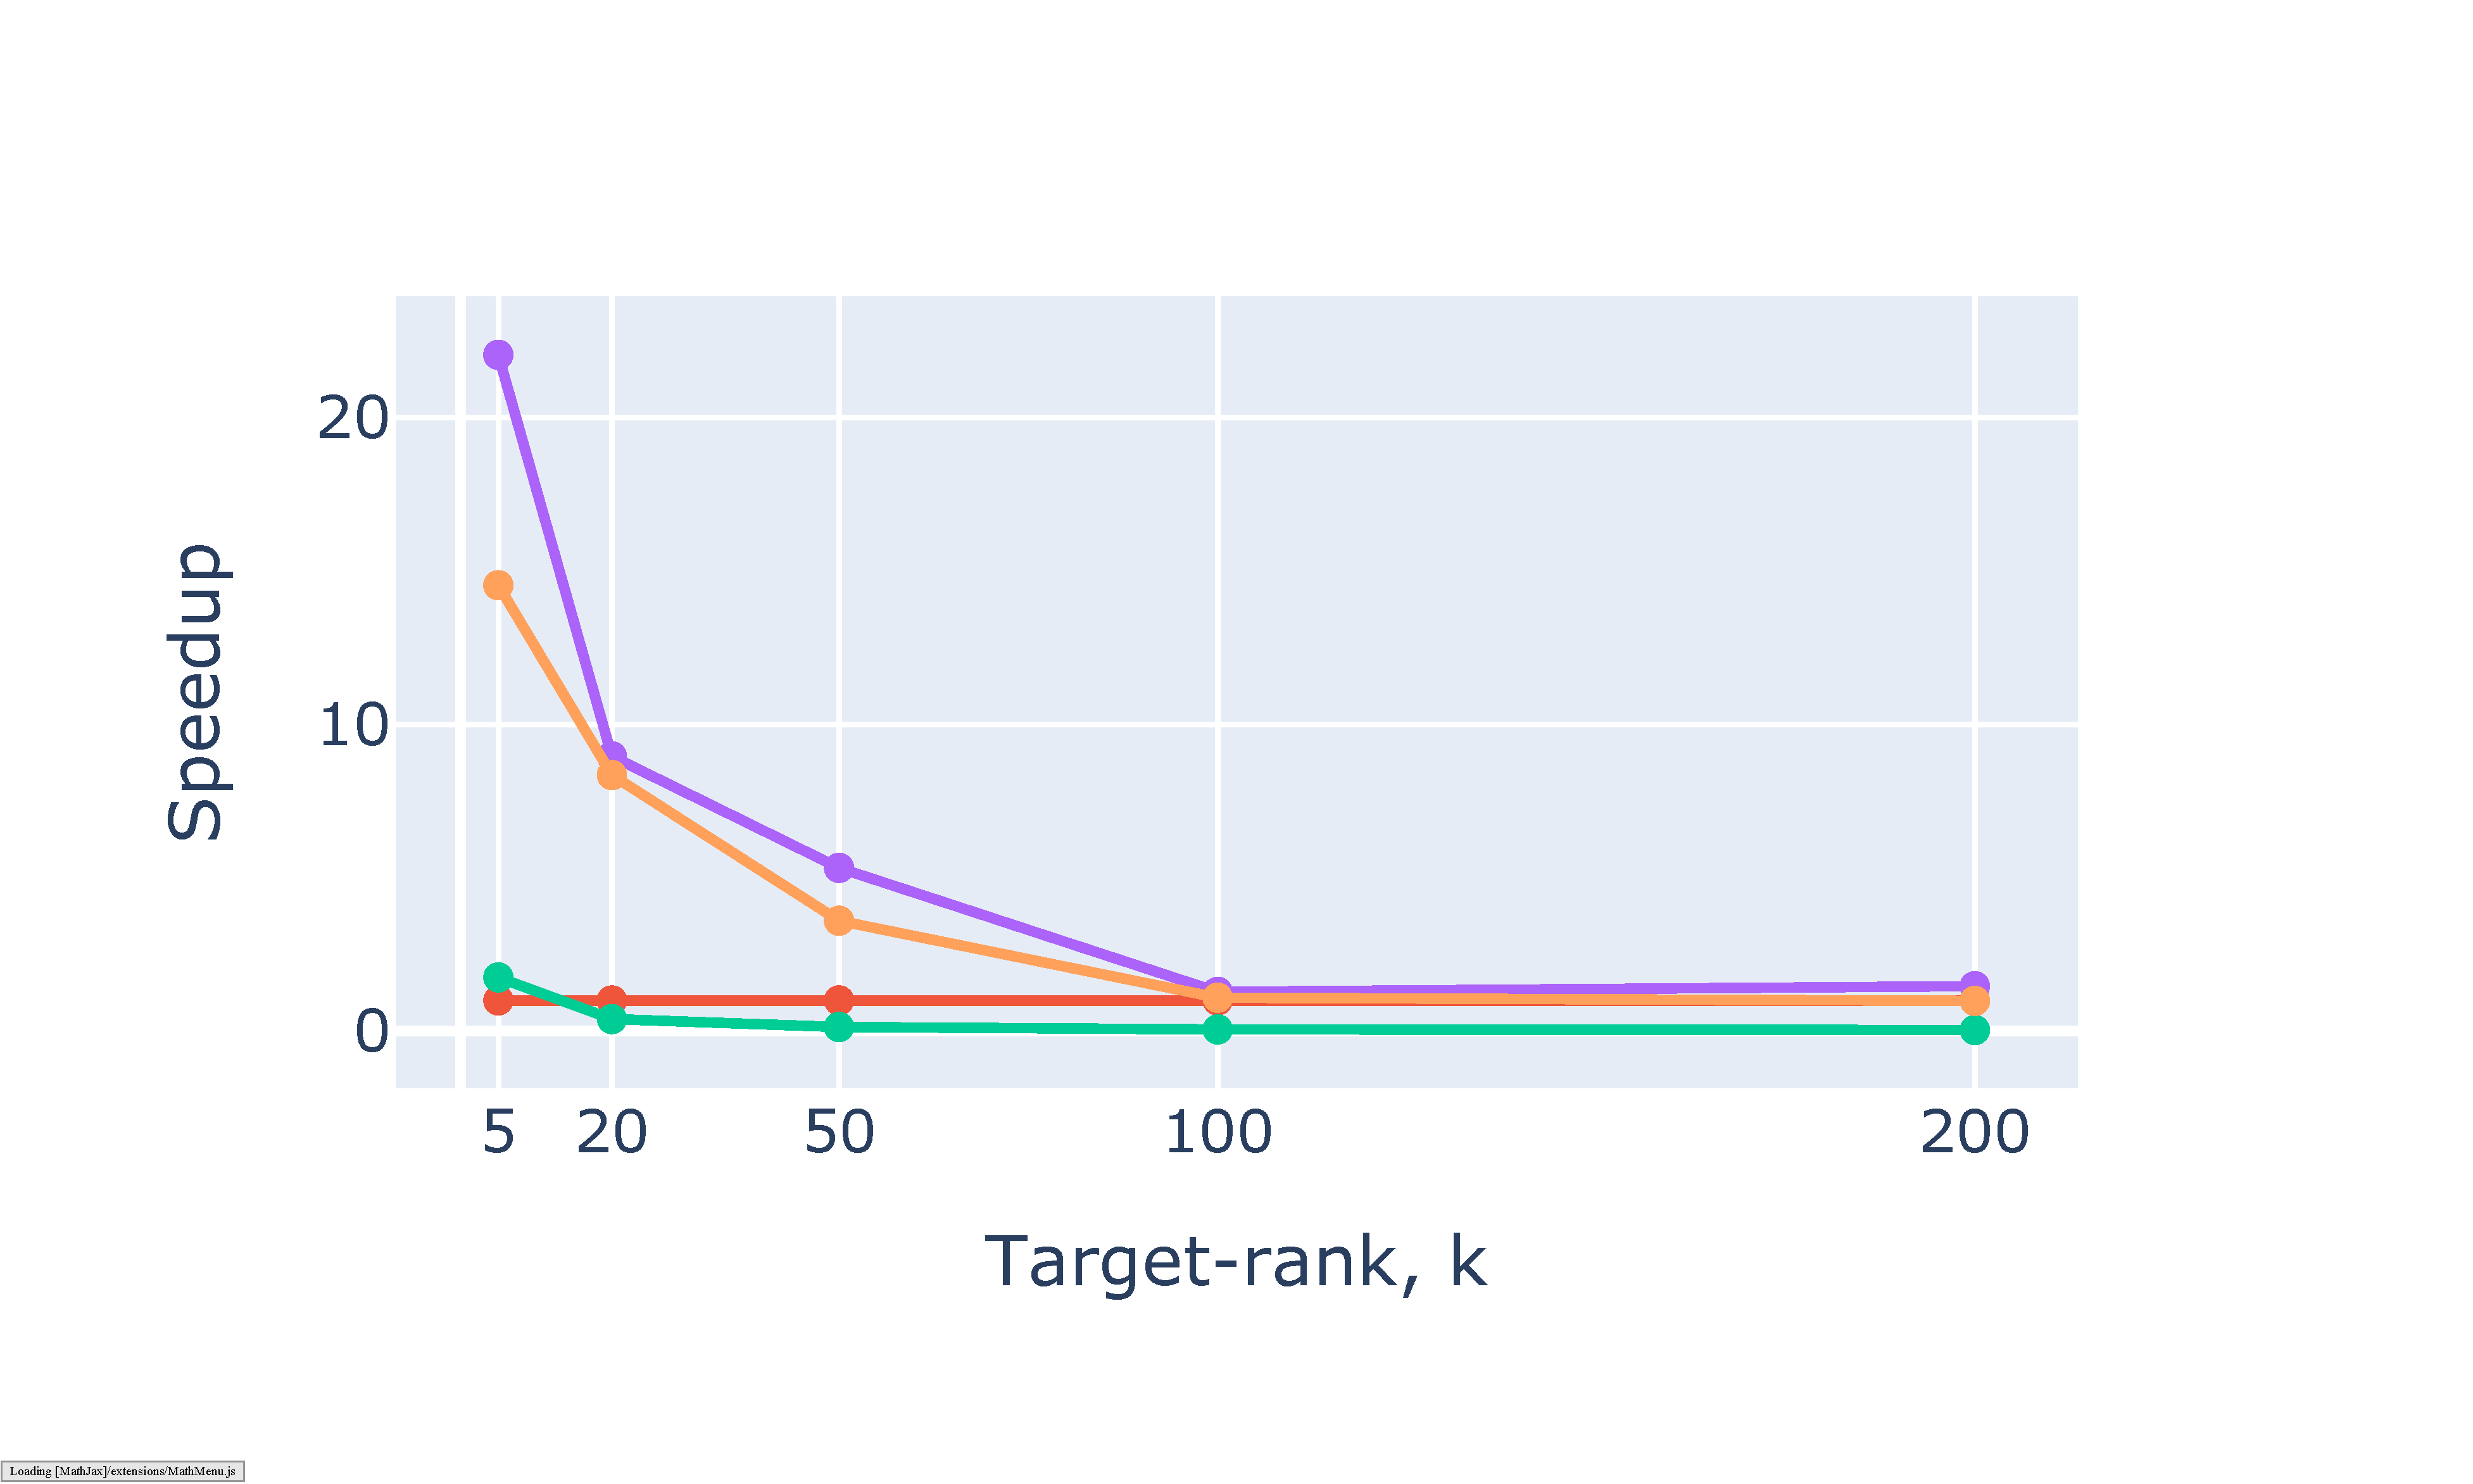
\includegraphics[width=\textwidth, trim={100 100 100 100}, clip]{Images/svd_speedup_sparse.pdf}
        \caption{Speedups.}
        \label{fig:speedups}
    \end{subfigure}
    \hfill
    % Third plot
    \begin{subfigure}[b]{0.31\textwidth}
        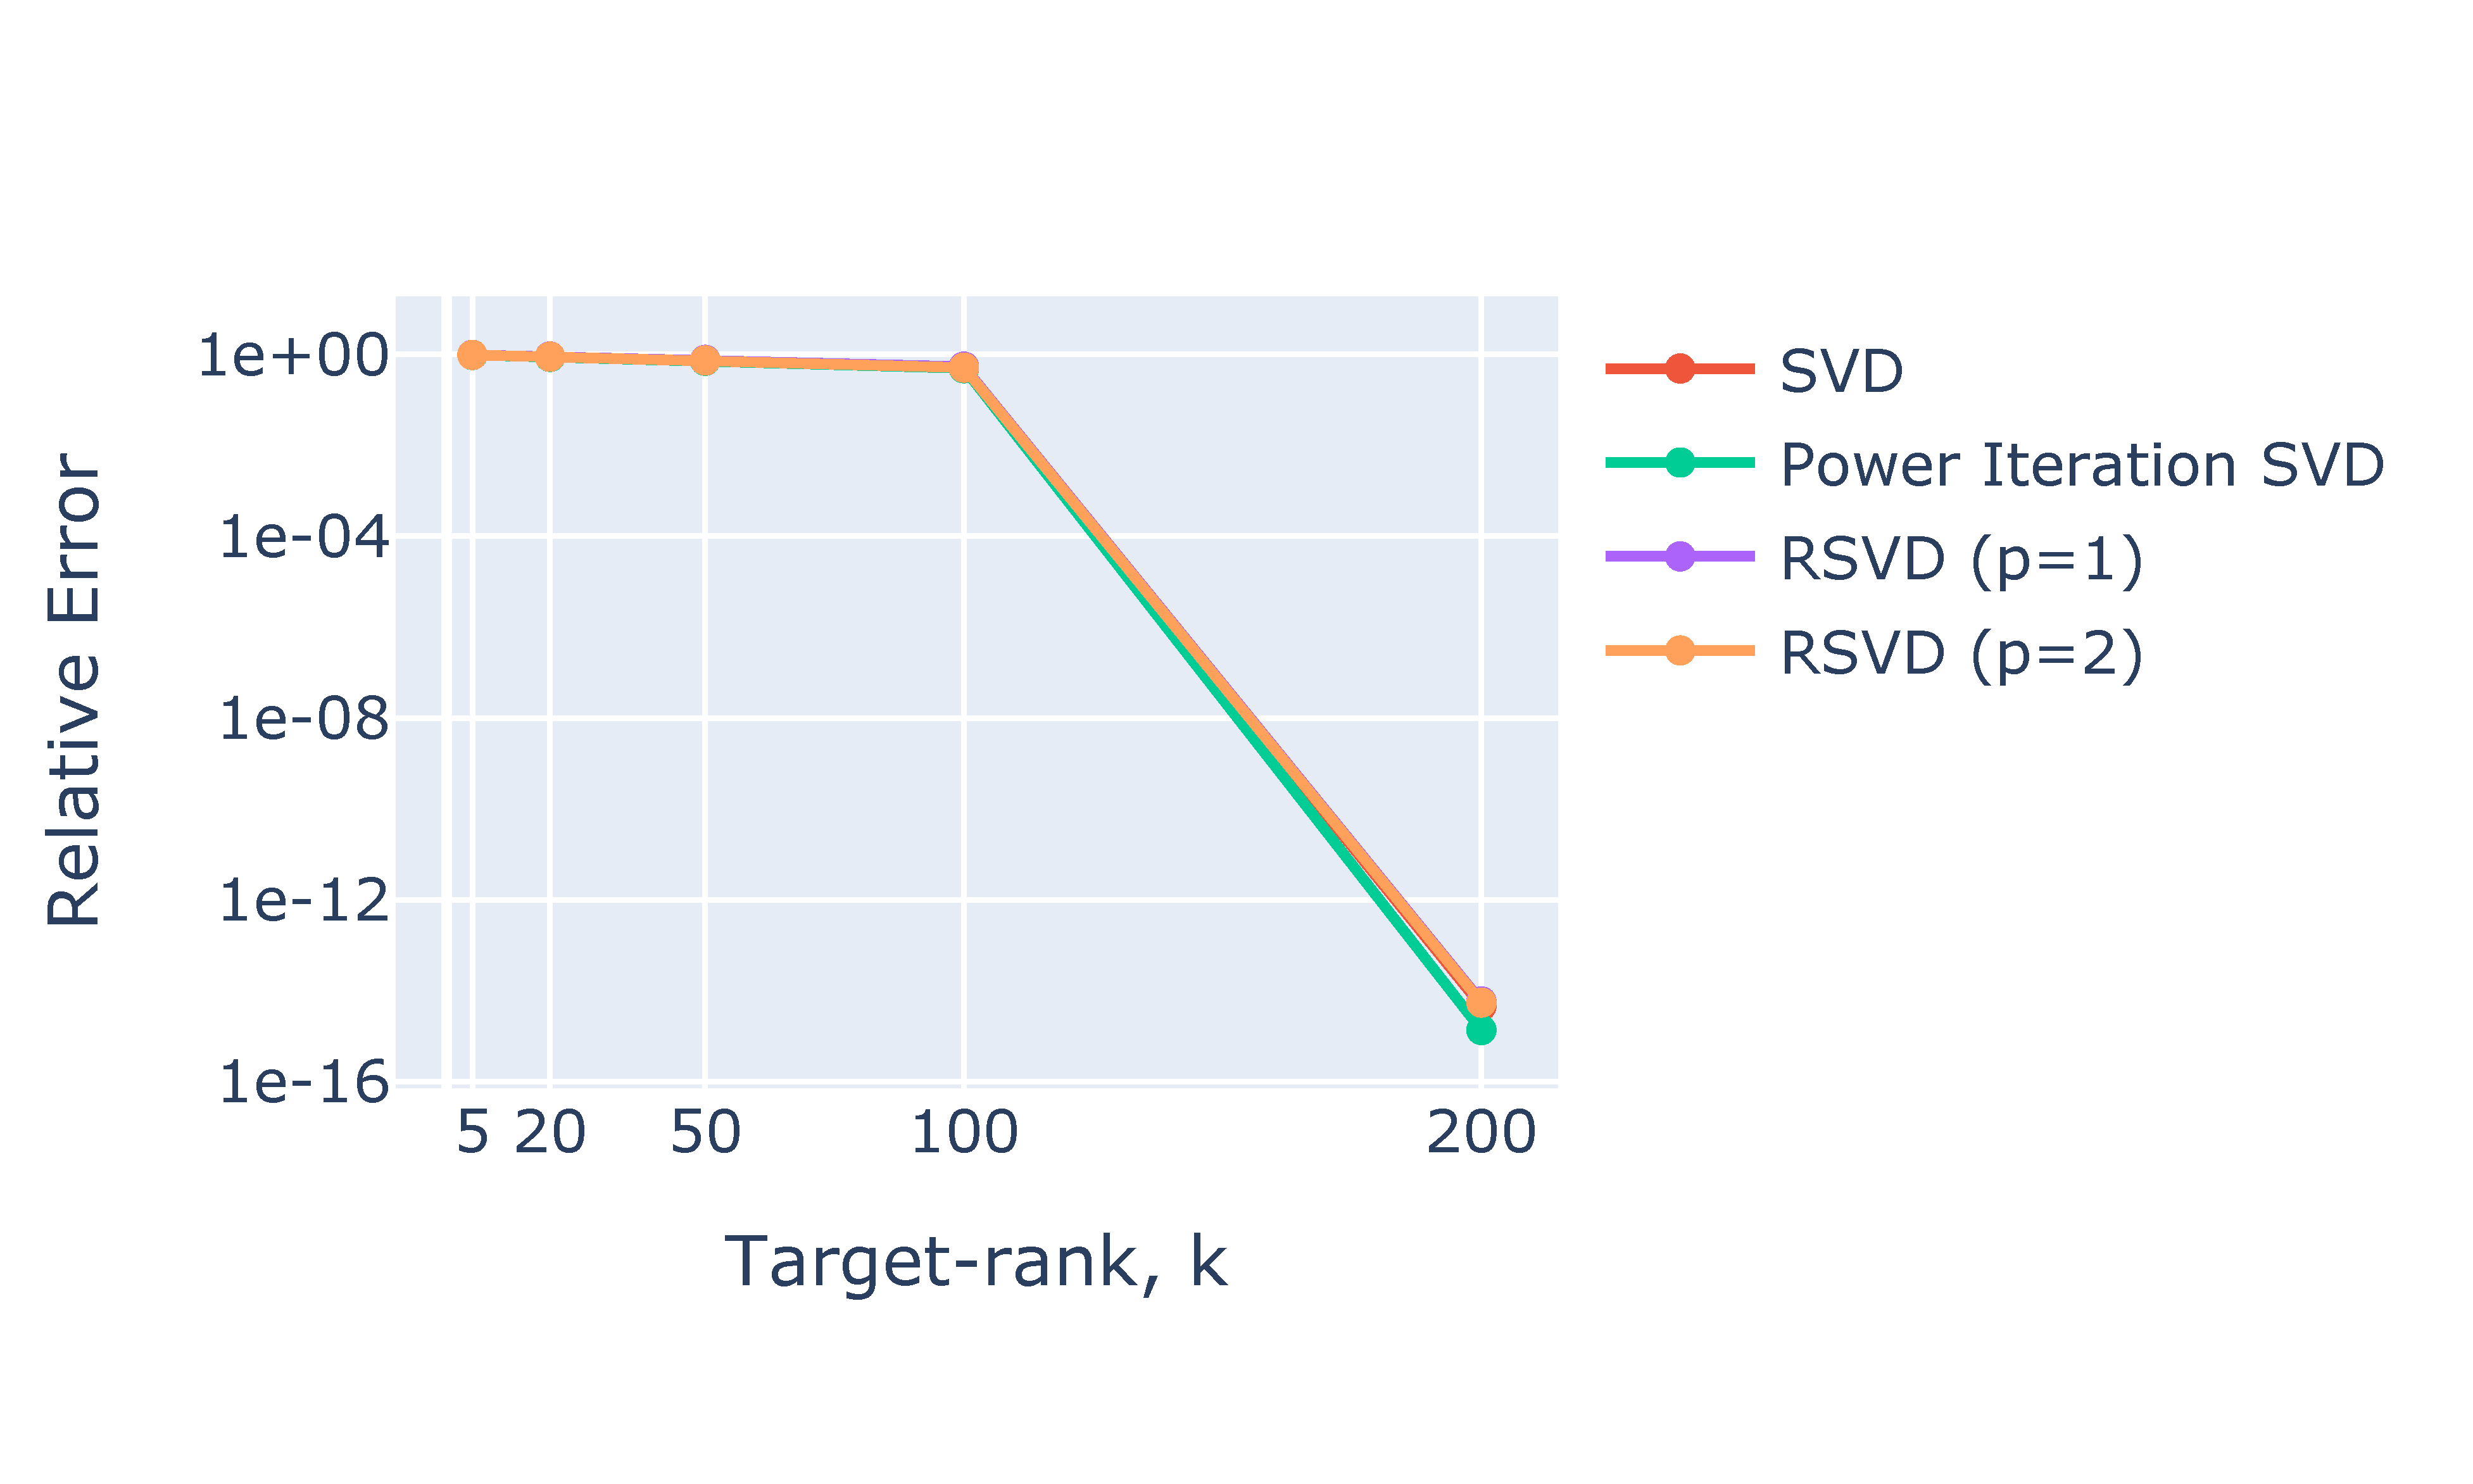
\includegraphics[width=\textwidth, trim={100 100 100 100}, clip]{Images/svd_error_sparse.pdf}
        \caption{Relative errors.}
        \label{fig:errors}
    \end{subfigure}

    \caption{Computational performance for a sparse $1000 \times 1000$ matrix}
    \label{fig:comparison}
\end{figure}

\subsection{Optimization technique}
\subsubsection*{Profiling}
A profiler is a program that allows to examine the performance of an executable and find possible bottleneck. Since I am using the macOS operating system, Valgrind is not available for the ARM64 architecture. Therefore, I chose to use Instruments for profiling, utilizing the following command-line tool for profiling:
\begin{minted}[fontsize=\small, linenos, frame=single]{bash}
xcrun xctrace record --template 'Time Profiler' --launch ./rsvd_dense_profiling
\end{minted}
Fig \ref{fig:profiler_rSVD} shows the result. For my 8-core CPU, the image shows that \texttt{OpenMP} successfully started 8 threads, with the main thread out, each thread sharing about 10\%-12\% of the workload. Matrix multiplication is also shown to be the bottleneck of this implementation.

\begin{figure}[H]
    \centering
    % left figure
    \begin{subfigure}[b]{0.48\textwidth}
        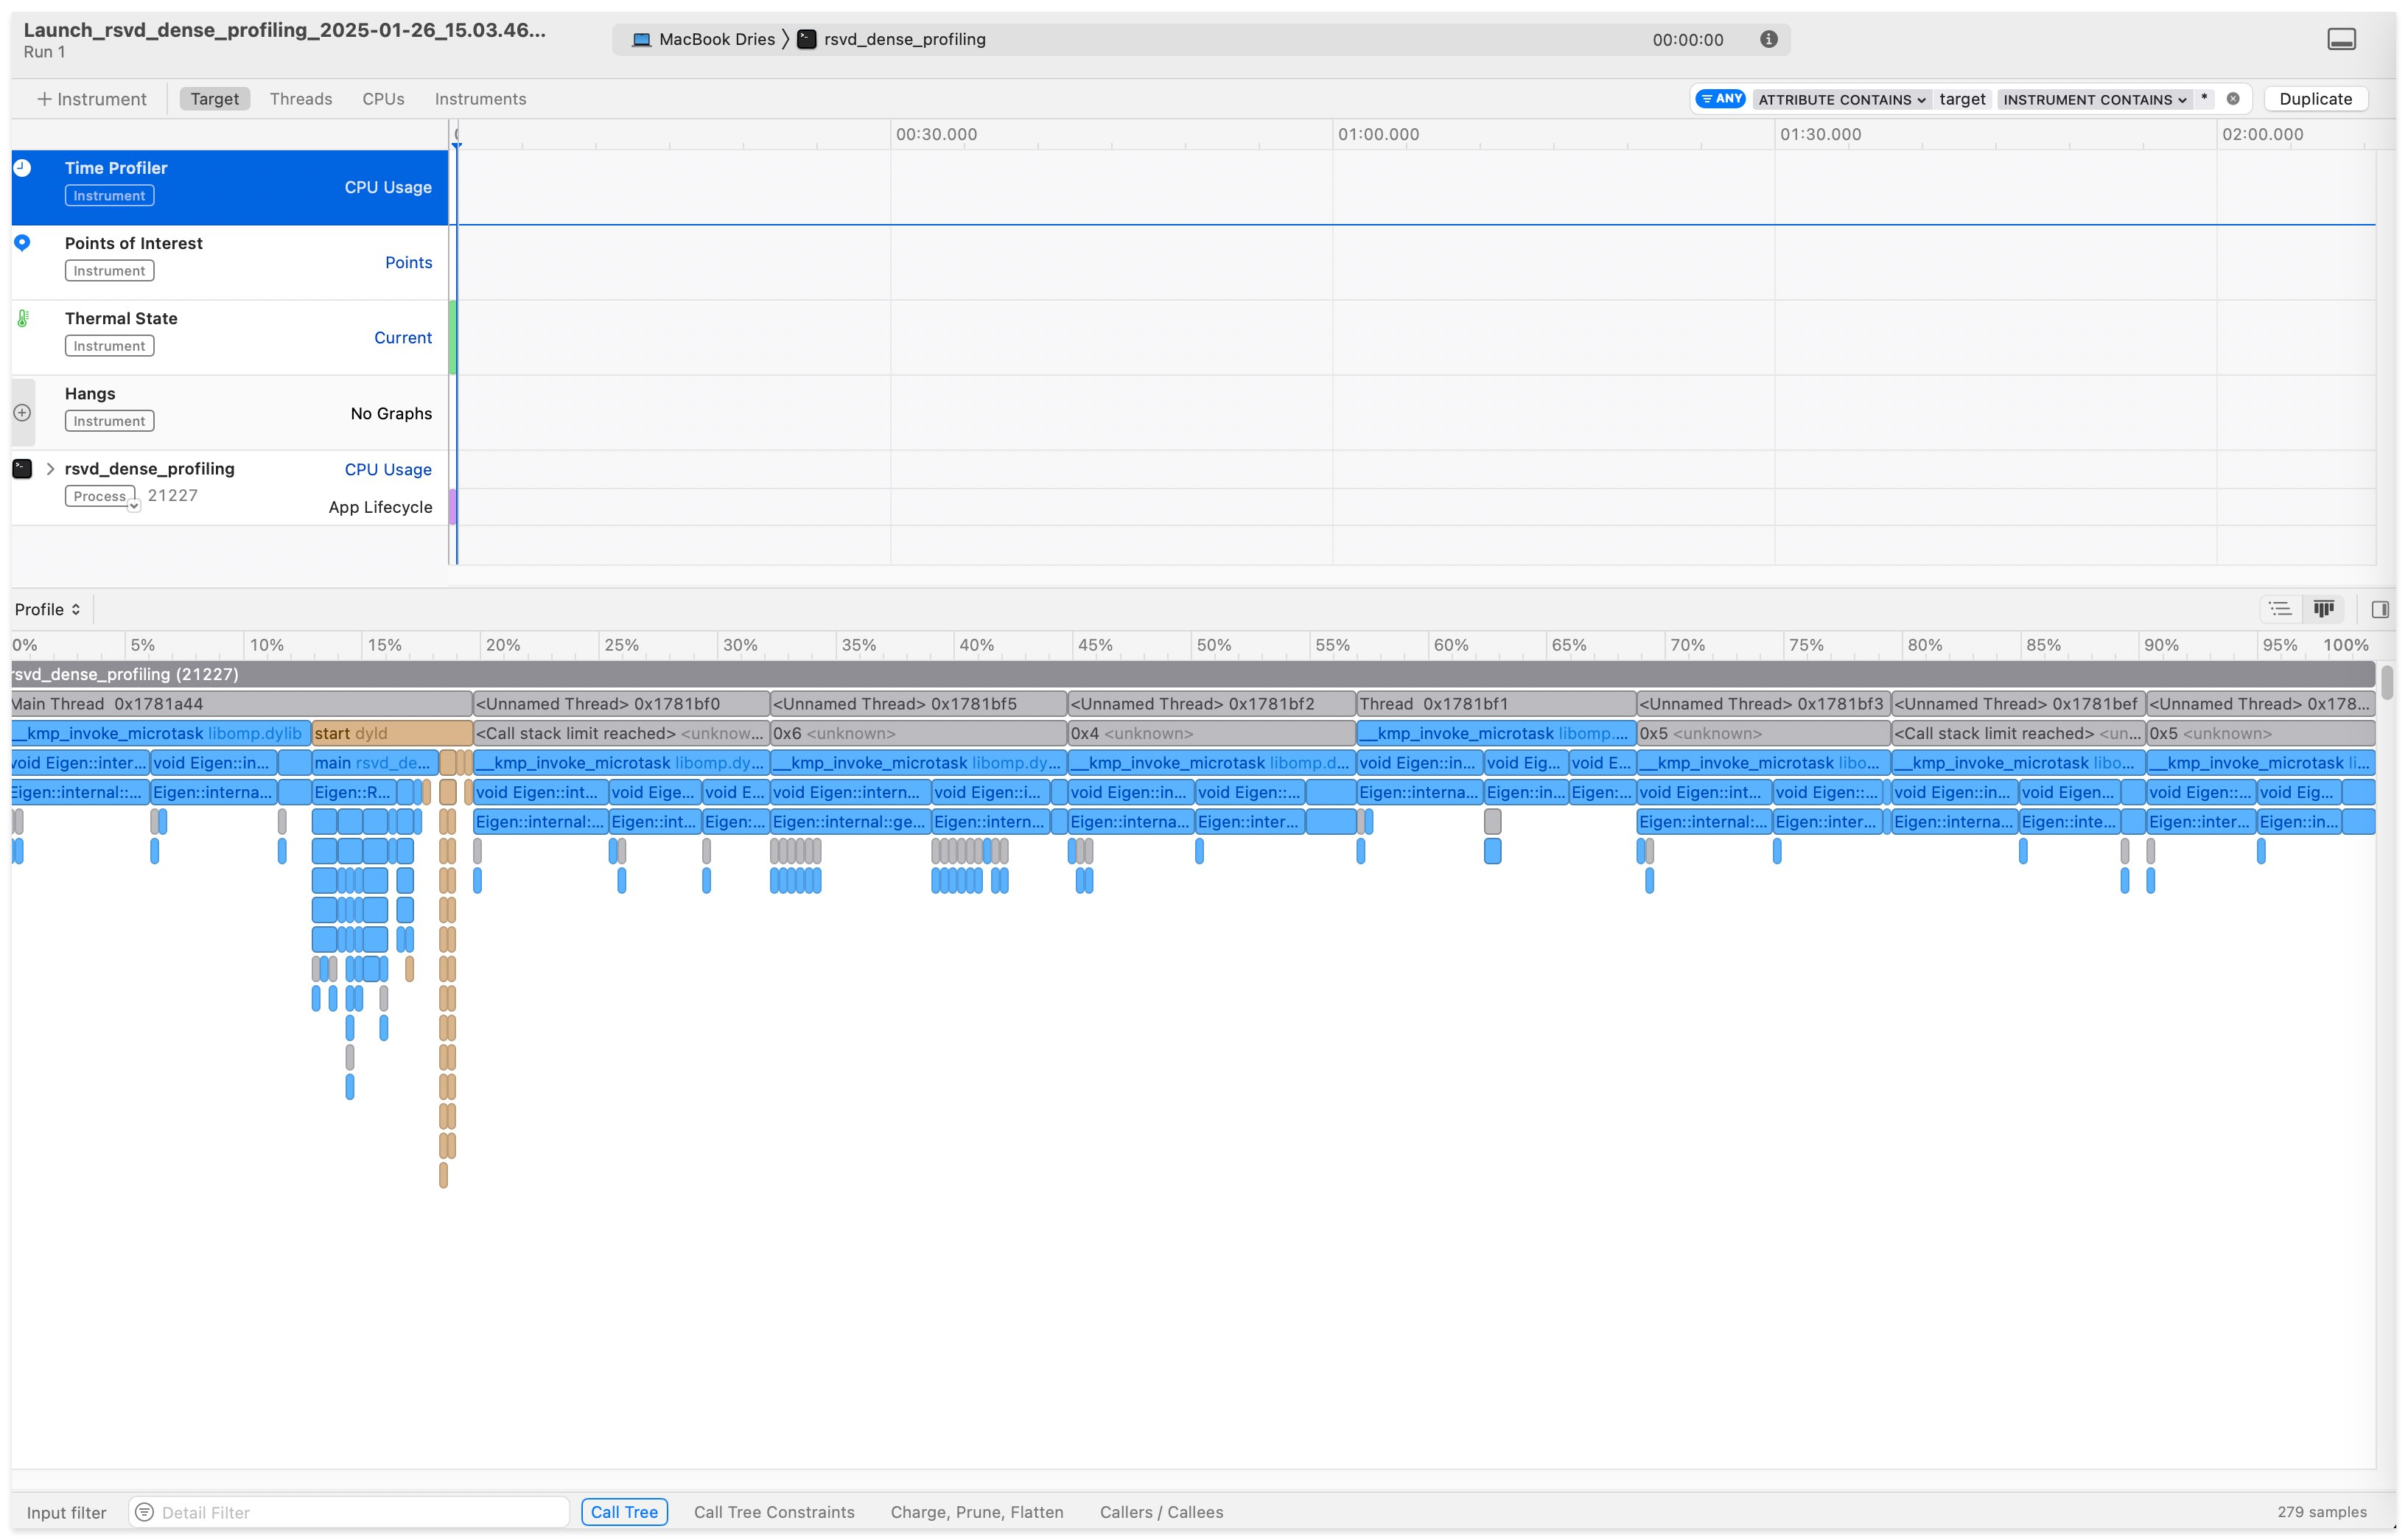
\includegraphics[width=\textwidth]{Images/svd_profiling.jpg}
        \caption{Profile.}
    \end{subfigure}
    % right figure
    \begin{subfigure}[b]{0.48\textwidth}
        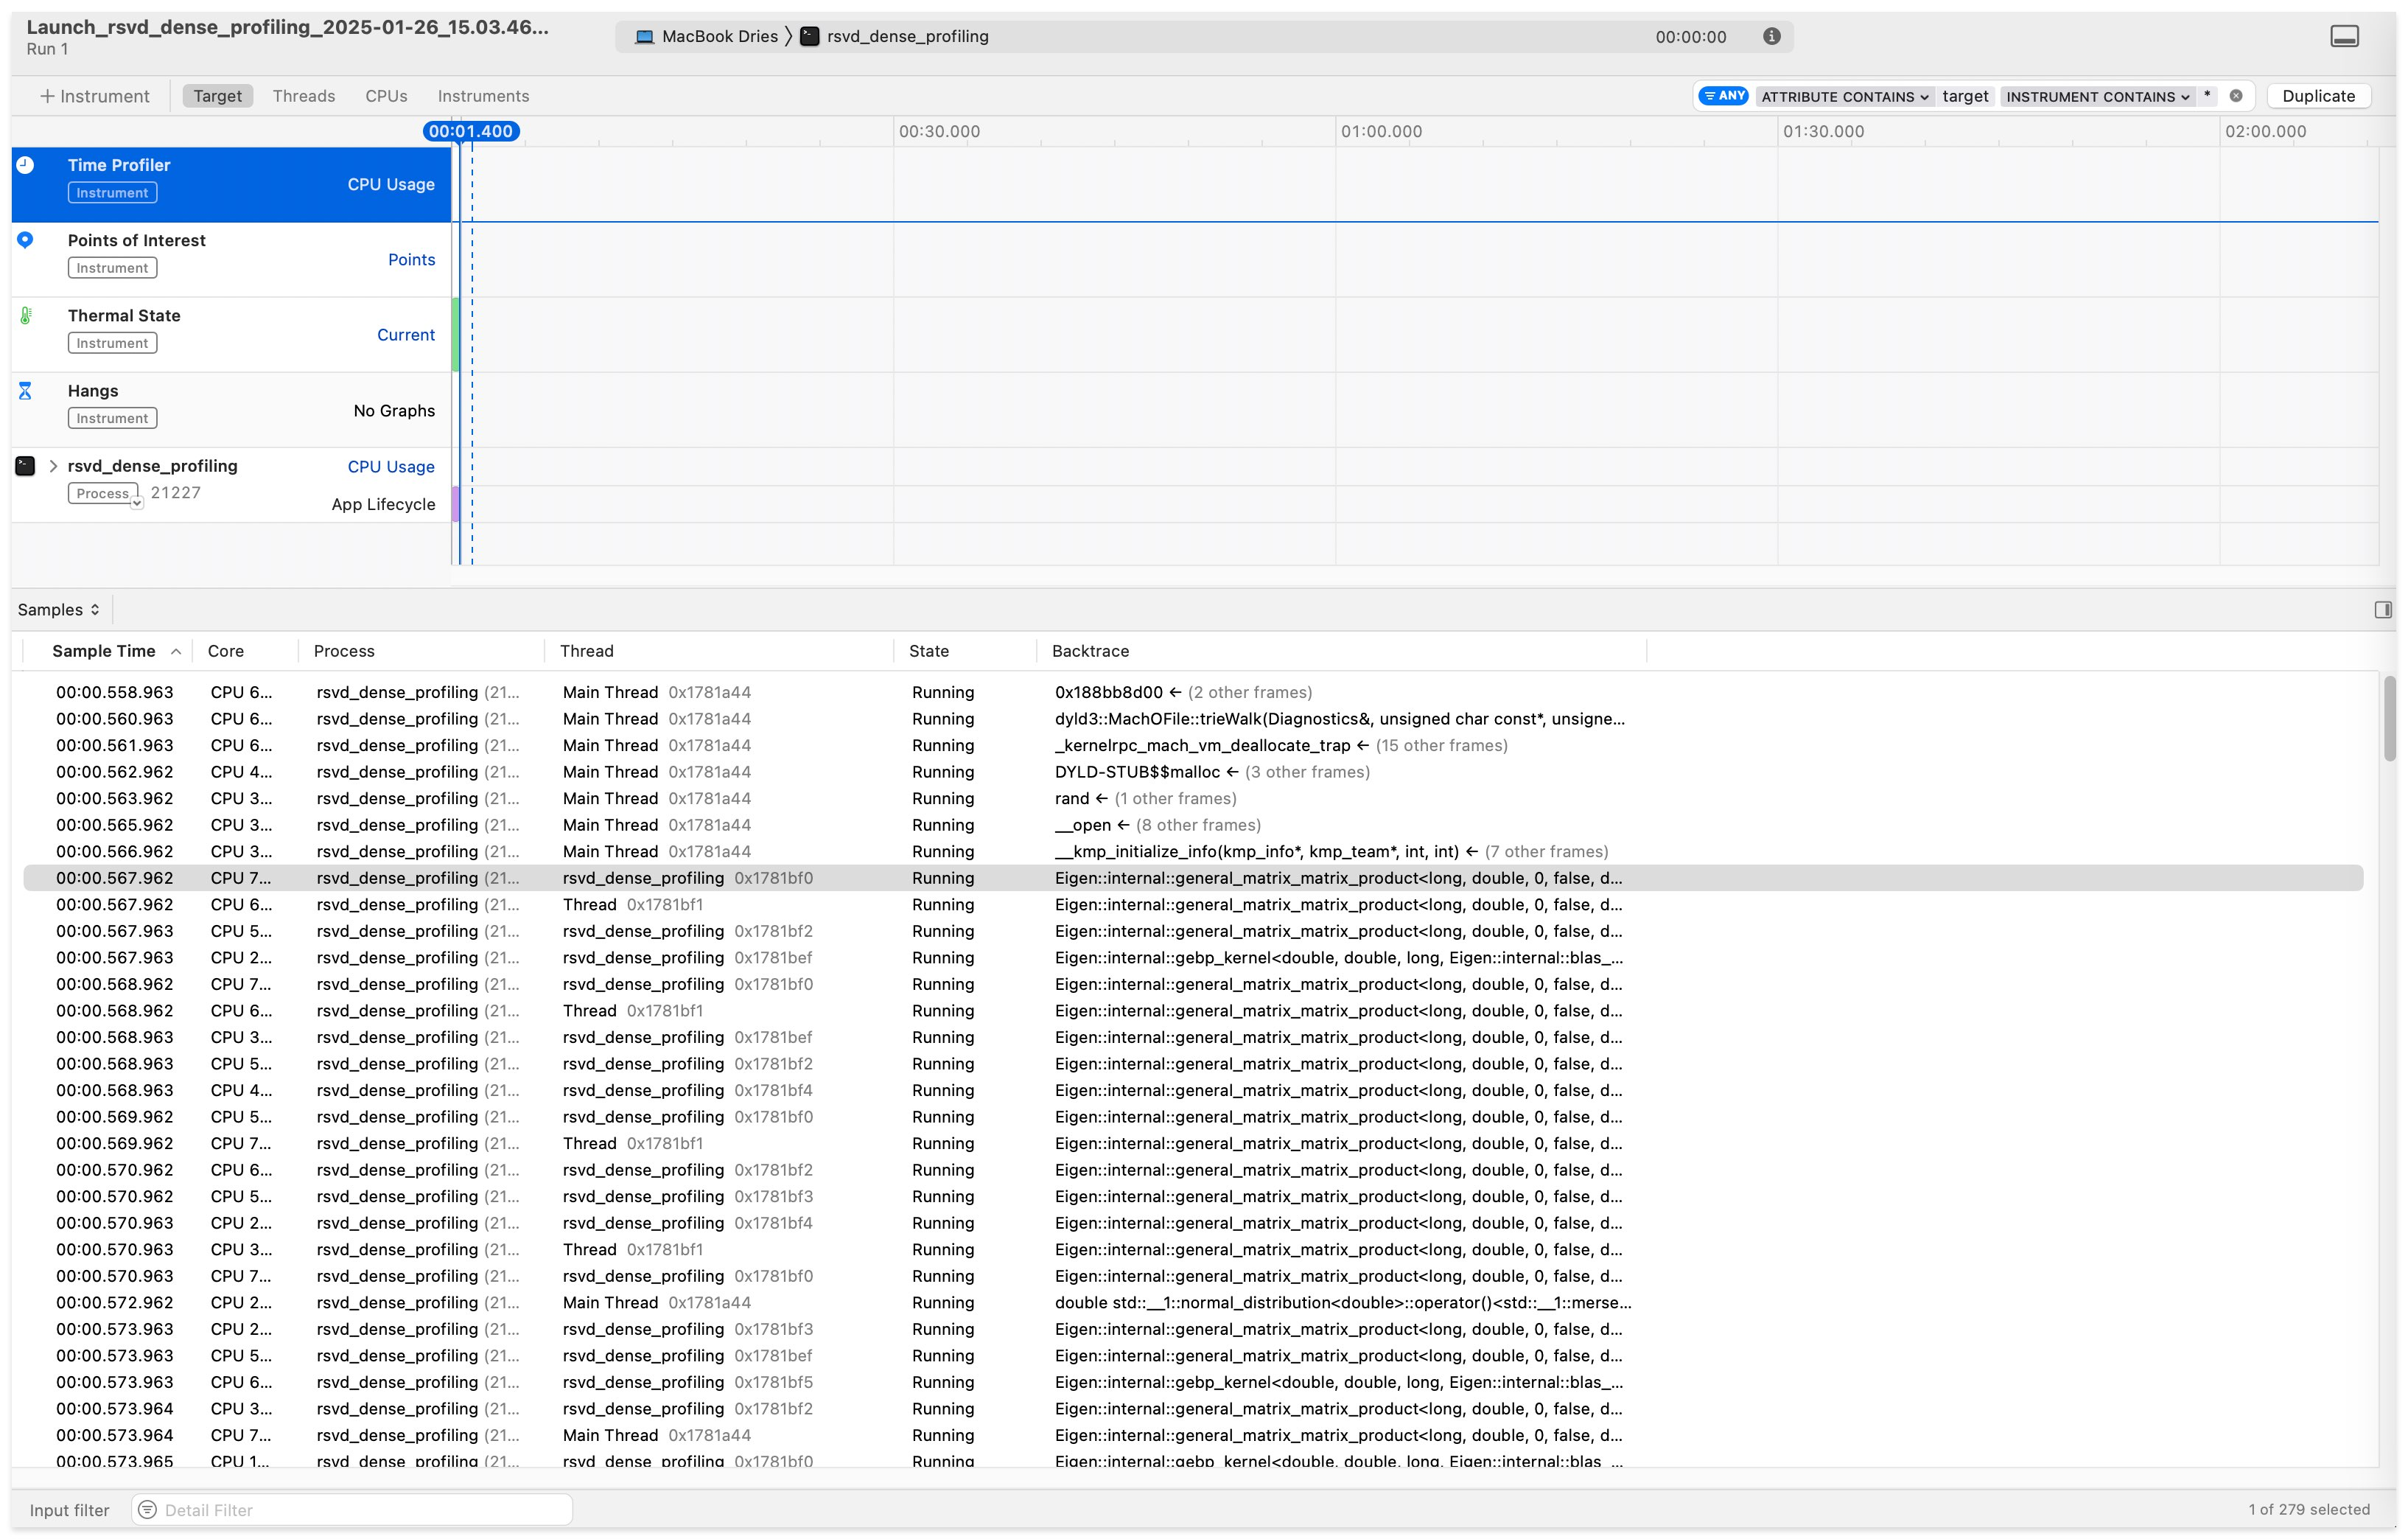
\includegraphics[width=\textwidth]{Images/svd_profiling1.jpg}
        \caption{Samples.}
    \end{subfigure}
    \caption{Profile for dense rsvd}
    \label{fig:profiler_rSVD}
\end{figure}
\subsubsection*{Parallelism}
We use multiple threading for parallelization. For Eigen, the parallelization of matrix multiplication can be achieved by adding the following compilation directive, and we have enabled \textbf{level 03 optimization}, as well as using \textbf{-march=native} to instruct the compiler to generate optimized machine code based on the current hardware architecture.
\begin{minted}[fontsize=\small, linenos, frame=single]{cmake}
add_executable(dense_svd dense_svd.cpp)
target_link_libraries(dense_svd PRIVATE Eigen3::Eigen)
target_link_libraries(dense_svd PRIVATE OpenMP::OpenMP_CXX)
target_compile_options(dense_svd PRIVATE -O3 -march=native)
\end{minted}

\subsubsection*{Sorting}
The key optimization is sorting the nonzero row indices in descending order before applying the rotations. Eliminates larger-indexed elements first, reducing interference in subsequent steps. Reduce redundant computations by systematically zeroing out elements from bottom to top.
\begin{minted}[fontsize=\small, linenos, frame=single]{cpp}
// Sort in descending order
std::sort(rowList.begin(), rowList.end(), std::greater<Index>());
\end{minted}

\subsubsection*{OpenBLAS}
\texttt{OpenBLAS} is an open-source implementation of the \texttt{BLAS} and \texttt{LAPACK} libraries. \texttt{Eigen} implements \texttt{OpenBLAS} acceleration by enabling the \texttt{\#define EIGEN\_USE\_BLAS} macro definition. On my computer (MacOS M1), the improvement of \texttt{OpenBLAS} for matrix operations is not significant, possibly due to the reasons of the chip architecture.
 
\subsubsection*{Memory access}
Memory access is also one of the bottlenecks. We found that Eigen does not access matrix elements as fast as expected. Therefore, in the Givens Rotation algorithm, since this algorithm needs to frequently access matrix elements, for the access that requires eliminating elements, we directly use pointers for access, which reduces the computation time by about 5 times.
\begin{minted}[fontsize=\small, linenos, frame=single]{cpp}
Scalar* data_ptr = matrix.data();
if constexpr (StorageOrder == RowMajor) {
    // RowMajor: (row, col) => row*cols + col
    for (Index row = 0; row < rows; ++row) {
        const Index offset_i = row * cols + i;
        const Index offset_k = row * cols + k;
        Scalar temp_i = data_ptr[offset_i];
        Scalar temp_k = data_ptr[offset_k];
        data_ptr[offset_i] = c * temp_i - s * temp_k;
        data_ptr[offset_k] = s * temp_i + c * temp_k;
    }
} else {
    // ColMajor: (row, col) => col*rows + row
    ...
    }
}
\end{minted}
\section{Applications}
In this section, we present some useful concrete applications of the RandomizedSVD algorithm.
\subsection{Image Compression}
Image compression is the process of \textbf{reducing the storage size of an image while preserving its visual quality as much as possible}. This can be achieved both with \textit{lossless} or \textit{lossy} algorithms. In the specific compression done with the Singular Value Decomposition, the algorithm used is lossy, in particular, it removes redundant or less significant information inside the image.\\ In mathematical terms, an image can be represented as a matrix of the same size as the image, where each entry corresponds to the intensity of a pixel (in grayscale) or a combination of 3 color channels (in RGB images).\\ 
Using Singular Value Decomposition (SVD), the matrix can be approximated as a \textbf{product of three smaller matrices}: 

\[A \approx U_k \Sigma_k (V_k)^T\]

Where k is the rank of the approximation. By retaining only the largest k singular values and their corresponding vectors, we can achieve a low-rank approximation of the image that captures its most essential features while discarding finer details. Instead of storing the whole image, we store only the compressed representation (meaning the three smaller matrices). When needed, the image can be reconstructed from these components, with a slight loss of detail proportional to the rank k. Randomized SVD accelerates this process by efficiently estimating the top k singular values and vectors using random sampling and projections, rather than computing the full decomposition. This makes RSVD particularly well-suited for compressing large images. 
\subsubsection{Code Explanation}
Brief explanation of the code: 
\begin{itemize}
    \item \textbf{Image Loading}: the program uses \textit{stb\_image} (which is a public domain image loader found at \url{http://nothings.org/stbto}) to load the input image, extracting its width, height and the number of channels. The pixel values are normalized to the range [0, 1] for numerical stability.
    \item \textbf{Grayscale Detection and Conversion}: if the image has three channels but is visually grayscale (meaning that all channels have equal intensity), it is reduced to a single grayscale channel for more efficient processing, eliminating redundant computations. This instance could happen due to compatibility reasons, or some applications' constraints, or for visual editing reasons. This specific instance is detected by a customized \textit{isGrayscaleRGB} function. Once the compression is done, the image will be brought back to its original number of channels.
    \item \textbf{Matrix Representation}: Each channel of the image is converted into an \textit{Eigen MatrixXd}, where rows and columns correspond to the pixel grid.
    \item \textbf{Compression via RSVD}: For each channel, the code computes a low-rank approximation of the image matrix using the Randomized SVD algorithm with the rank given as input by the user: \\
    \begin{minted}[fontsize=\small, linenos, frame=single]{cpp}
    rSVD.compute(channel_matrices[c], rank);
    compressed_channels[c] = rSVD.matrixU() * rSVD.singularValues().asDiagonal()
                             * rSVD.matrixV().transpose();
    \end{minted}
    Here, the rank is the most important parameter, specifying the number of singular values to retain and thus, controlling the level of compression.
    \item \textbf{Image Reconstruction}: The compressed matrices are scaled back to the [0, 255] range and converted into an \textit{std::vector<unsigned char>} for saving.
    \item \textbf{Saving the Compressed Image}: use \textit{stbi\_write\_png} (which is again a public domain image saver found at \url{http://nothings.org/stb} that writes out PNG/BMP/TGA/JPEG/HDR images to C stdio) to save the compressed image data to an output PNG file.
    \item \textbf{Relative Error Computation}: the program calculates the relative Frobenius norm error between the original and compressed image matrices for each channel:
    \begin{minted}[fontsize=\small, linenos, frame=single]{cpp}
    double original_norm = std::sqrt(channel_matrices[c].squaredNorm());
    double difference_norm = std::sqrt((channel_matrices[c] 
                             - compressed_channels[c]).squaredNorm());
    double relative_error = difference_norm / original_norm;
    total_relative_error += relative_error;
    \end{minted}
    Then, it computes the average total relative error across channels, allowing error comparison between compressed images with a different number of channels. This final value quantifies the compression accuracy.
    \item \textbf{Memory Usage Computation}: at last, the program calculates the memory used in terms of KBytes by the raw input matrix and by the three compressed matrices. With this values, it computes the memory compression ratio.
\end{itemize}
\begin{figure}[h!]
\centering
% Top row: Two images
\begin{subfigure}{0.3\textwidth}
    \centering
    \includegraphics[width=\textwidth]{Images/Image_Compression_images/image_grayscale.png}
    \caption{Original Image \\}
\end{subfigure}
\hspace{0.05cm}
\begin{subfigure}{0.3\textwidth}
    \centering
    \includegraphics[width=\textwidth]{Images/Image_Compression_images/compressed_image_200.png}
    \caption{Rank=200}
\end{subfigure}

\vspace{0.5cm} % Adds vertical space between the rows

% Bottom row: Three images
\begin{subfigure}{0.3\textwidth}
    \centering
    \includegraphics[width=\textwidth]{Images/Image_Compression_images/compressed_image_100.png}
    \caption{Rank=100}
\end{subfigure}
\hspace{0.05cm}
\begin{subfigure}{0.3\textwidth}
    \centering
    \includegraphics[width=\textwidth]{Images/Image_Compression_images/compressed_image_50.png}
    \caption{Rank=50}
\end{subfigure}
\hspace{0.05cm}
\begin{subfigure}{0.3\textwidth}
    \centering
    \includegraphics[width=\textwidth]{Images/Image_Compression_images/compressed_image_10.png}
    \caption{Rank=10}
\end{subfigure}

\caption{Compression results with different ranks}
\label{fig:compression_comparison}
\end{figure}


\subsubsection{Results Analysis}
The results were evaluated both visually and analytically. In particular, we compared the different results using the \textbf{relative error} computed as:

\[\text{Relative Error} = \frac{||A-A_{\text{compressed}}||_F}{||A||_F}\]
Where the F-norm (\textit{Frobenius norm}) is defined as:
\[\|A\|_F = \sqrt{\sum_{i=1}^m \sum_{j=1}^n |a_{ij}|^2}\]
And the \textbf{memory compression ratio}, computed as:

\[\text{Compression Ratio (CR)} = \frac{\text{bytes of input image}}{\text{total bytes of } U_k, \Sigma_k \text{ and } (V_k)^T} \]
The formula used was chosen to be independent of the memory saving format of both input and output, it computes the raw matrices sizes to understand how rSVD influences them. \\
\textbf{Figure} \textbf{\ref{fig:compression_comparison}} displays a gray scale image of size 4000 x 6000 with 3 channels along with its compressed versions using different ranks. \textbf{Table \ref{tab:compression}} shows how increasing the rank also reduces the relative error, this makes sense because we are keeping more information about the matrix. However, if with smaller ranks the CR is larger than 1, meaning the compression is effective memory-wise, performed tests have proved that, after a certain rank (around 10\% of the image width), the CR goes under 1, meaning the compressed matrices actually occupy more memory than the input image. This happens because the memory used by the compressed matrices grows linearly for U\_k and V\_k transposed while it grows quadratically for Sigma\_k. However, our evaluation doesn't take into account the compression power of image saving formats. For example, using data storage formats after rSVD compression like CSR, CSC, HDF5 or MM that are specific for the sparse and low-rank matrices created by rSVD, would probably increase the threshold rank. The \textbf{limitations of rSVD}, and SVD, as cited in \cite{WANG2023102182}, come from the fact that it is \textbf{inherently redundant}, because \textit{U} and \textit{V} are \textit{r-rank orthonormal}, inherently including constraints that prevent SVD from deeper compression and even making it frustrated as the data fidelity is strictly required. In this same paper, the solution found is to enhance the power of the SVD algorithm using \textbf{E-SVD}, which includes entropy coding like the JPEG compression format. Other papers like \cite{BRYT2008270}, find a better solution in \textbf{K-SVD}, which is an iterative algorithm that extends SVD by learning a sparse and adaptive dictionary for signal representation. 

\begin{table}[h]
    \centering
    \begin{tabular}{|c|c|c|}
        \hline
        Rank & Relative Error & Memory Compression Ratio \\
        \hline
         10 &0.160166  &29.97  \\
        \hline
         50 &0.123699  &5.97015  \\
        \hline
         100 &0.0741506  &2.9703  \\
        \hline
        200 &0.050169 &1.47059 \\
        \hline
        300 &0.030199 &1.05408 \\
        \hline
        400 &0.024068 &0.9739 \\
        \hline
    \end{tabular}
    \caption{Table showing rank, relative error, and memory compression ratio of various test compressions performed with rSVD}
    \label{tab:compression}
\end{table}

From a \textbf{visual point of view}, tests have proven that:
\begin{itemize}
    \item Using a rank \textit{below 5-10\%} visually degrades the quality of the image and can introduce artifacts. Take into account that the ability to recognize compression mainly depends on how big the displayed image is (roughly speaking, if we zoom into the image, compression is much more obvious), so, depending on the use we want to make of the compressed image, we could be satisfied even with lower ranks.
    \item Using a rank \textit{above 15\%} outputs a good quality image, making compression hard to spot.
\end{itemize}


\subsubsection{Note}
These results strongly depend on the specific structure of the image to compress, in particular on:
\begin{itemize} [label=-]
    \item \textbf{Redundancy}: how much pixels are correlated with each other. It can be \textit{spatial} (smooth regions, large areas of similar colors, ...) or \textit{spectral} (highly correlated channels). More redundant images are easier to compress because we can exploit correlation to make predictions.
    \item \textbf{Image Complexity}: it relates with how much the image structure is predictable, objects that have sharp edges, images with small details and fine textures or high color variability are harder to compress.
    \item \textbf{Noise}: strongly related to image complexity, if an image is noisy, it's less predictable because noise appears as random and with high-frequency.
\end{itemize}
What we can focus on, is the sufficient starting efficiency of the rSVD Image Compression implementation presented, giving a good starting point for further studies on better compression algorithms or versions of SVD and it's randomized counterpart.


\subsection{Handwritten Numbers Recognition}
We implemented a handwritten digit recognition system using the MNIST dataset and RandomizedSVD for dimensionality reduction. The MNIST dataset consists of 28x28 pixel grayscale images of handwritten digits (0-9), making each image a 784-dimensional vector. Our implementation combines dimensionality reduction through rSVD with nearest neighbor classification.

\subsubsection{Implementation Details}
The system consists of three main components:

\begin{itemize}
    \item \textbf{Data Loading}: The \texttt{MNISTLoader} class handles loading and preprocessing of the MNIST dataset, converting the binary format into normalized Eigen matrices.
    \item \textbf{Dimensionality Reduction}: Using rSVD through our PCA implementation to reduce the 784-dimensional images to a lower-dimensional space while preserving essential features.
    \item \textbf{Classification}: A nearest neighbor classifier that works in the reduced dimensional space to predict digit labels.
\end{itemize}

The training process involves:
\begin{enumerate}
    \item Computing the mean of the training data
    \item Centering the data by subtracting the mean
    \item Applying rSVD-based PCA to obtain the projection matrix
    \item Projecting training data into the reduced space
\end{enumerate}

For prediction, new images are:
\begin{enumerate}
    \item Centered using the training mean
    \item Projected into the reduced space
    \item Classified using nearest neighbor comparison with the reduced training data
\end{enumerate}

\subsubsection{Code Explanation}
The core implementation consists of training and prediction phases. During training, we first load and normalize the MNIST data, then use PCA for dimensionality reduction:

\begin{minted}[fontsize=\small, linenos, frame=single]{cpp}
// Load and normalize MNIST data to [0,1]
auto [images, labels] = MNISTLoader::loadMNISTData(images_path, labels_path);

// Reduce dimensions using PCA
Eigen::PCA pca;
pca.computeByRSVD(training_data, num_components_, num_components_);
reduced_training_data_ = pca.reducedMatrix();
\end{minted}

For prediction, we use nearest neighbor classification in the reduced dimensional space to identify digits.

\subsubsection{Results Analysis}
We conducted experiments using 10,000 training images and 1,000 test images, varying the number of components used in the dimensionality reduction. Table \ref{tab:mnist_accuracy} shows the classification accuracy for different numbers of components:

\begin{table}[h]
    \centering
    \begin{tabular}{|c|c|}
        \hline
        Number of Components & Accuracy \\
        \hline
        2 & 37.9\% \\
        4 & 58.1\% \\
        8 & 85.1\% \\
        16 & 92.3\% \\
        32 & 93.7\% \\
        64 & 93.3\% \\
        128 & 93.1\% \\
        256 & 92.7\% \\
        \hline
    \end{tabular}
    \caption{MNIST Classification Accuracy vs Number of Components}
    \label{tab:mnist_accuracy}
\end{table}

Key observations from the results:

\begin{itemize}
    \item \textbf{Rapid Improvement}: Accuracy improves dramatically from 37.9\% with 2 components to 85.1\% with just 8 components, showing that even a small number of components can capture significant discriminative features.
    
    \item \textbf{Optimal Performance}: Peak accuracy of 93.7\% is achieved with 32 components, suggesting this is the optimal balance between dimensionality reduction and information preservation.
    
    \item \textbf{Diminishing Returns}: Beyond 32 components, accuracy slightly decreases, possibly due to overfitting or the inclusion of noise components. This demonstrates that more components don't always lead to better performance.
    
    \item \textbf{Efficiency}: The system achieves over 92\% accuracy while reducing dimensionality from 784 to just 16 dimensions, representing a 98\% reduction in data dimensionality.
\end{itemize}

The implementation also includes a single image prediction test that successfully identifies individual digit images, demonstrating the practical applicability of the system for real-world handwritten digit recognition tasks.

These results demonstrate that rSVD can effectively reduce the dimensionality of image data while maintaining the discriminative features necessary for accurate classification. The high accuracy achieved with relatively few components highlights the efficiency of our implementation in capturing the essential characteristics of handwritten digits.

\subsection{Principal Component Analysis (PCA)}
\textbf{Principal Component Analysis (PCA)} is a dimensionality reduction technique widely used in data science, machine learning and statistics. \textbf{It transforms high-dimensional data into a lower-dimensional form while preserving as much of the original information as possible}.

Originally, PCA was achieved by obtaining a covariance matrix. Where covariance is defined as:

\begin{equation}
    cov(x,y)=\frac{\sum_{i=1}^n(x_i-\bar{x})\left(y_i-\bar{y}\right)}{n-1}
\end{equation}
and then we can get covariance matrix:
\begin{equation}
    C=
\begin{bmatrix}
cov(x,x) & cov(x,y) \\
cov(x,y) & cov(y,y)
\end{bmatrix}
\end{equation}
because $\bar{x}$ and $\bar{y}$ equal to 0 with centralization. we can transform equation to:
\begin{equation}
        C=
\begin{bmatrix}
\frac{\sum_{i=1}^nx_i^2}{n-1} & \frac{\sum_{i=1}^nx_iy_i}{n-1} \\
\frac{\sum_{i=1}^nx_iy_i}{n-1} & \frac{\sum_{i=1}^ny_i^2}{n-1}
\end{bmatrix}
\end{equation}
convert it to the matrix multiplication form:

\begin{equation}
    =\frac{1}{n-1}
        \begin{bmatrix}
        x_1 & x_2 & x_3 & x_4 \\
        y_1 & y_2 & y_3 & y_4
        \end{bmatrix}
        \begin{bmatrix}
        x_1 & y_1 \\
        x_2 & y_2 \\
        x_3 & y_3 \\
        x_4 & y_4
        \end{bmatrix}
\end{equation}
finally we can get:
\begin{equation}
    C=\frac{1}{n-1}D^\mathrm{T}D
\end{equation}
$D$ is our data matrix. In order to preserve more information of our data matrix, when we want to get principal component  of matrix,  we need to get eigenvector of covariance matrix and sorting it with eigenvalue. In the meantime, we have this equation in SVD decomposition:
\begin{equation}
    D^\mathrm{T}D=VLV^\mathrm{T}
\end{equation}
it is equivalent to performing an SVD decomposition on $D$ matrix. $V$ matrix is  consisted by covariance eigenvector. $L$ matrix is a diagonal matrix and the value in the diagonal is the square of eigenvalue. In this way, we can perform PCA by SVD decomposition instead of computing covariance matrix which is more complexity. In this thesis, we are discoursing about RSVD, which can get better performance than SVD. 
\subsubsection{Code Explanation}
Brief explanation of the code: 
\begin{itemize}
    \item \textbf{Data centralization}: In order to get best direction to project our data, we need to centralize our data.
\begin{minted}[fontsize=\small, linenos, frame=single]{cpp}
    Eigen::VectorXd mean = data.colwise().mean();  // get mean value of each col
    Eigen::MatrixXd centered = data.rowwise() - mean.transpose();
\end{minted}
    \item \textbf{Performing RSVD decomposition}: We need to perform RSVD decomposition on our centered matrix to get $V$ matrix. where rank is preferably equal to final dimension and can't be smaller than dimension.
\begin{minted}[fontsize=\small, linenos, frame=single]{cpp}
    Eigen::RandomizedSVD<Eigen::MatrixXd> rSVD;
    rSVD.compute(centered, rank);
\end{minted}
    \item \textbf{Get principal component}: Get previous component of $V$ matrix, the number is equal to our target dimension of data.
\begin{minted}[fontsize=\small, linenos, frame=single]{cpp}
    Eigen::MatrixXd principal_components = rSVD.matrixV().leftCols(dimension);
\end{minted}
    \item \textbf{Data projection}: Finally we do matrix multiplication to project our data on target dimension.
    \begin{minted}[fontsize=\small, linenos, frame=single]{cpp}
    this->reducedMat = centered * principal_components;
\end{minted}

\end{itemize}
\subsubsection{Results Analysis}
We have performed variant implementation of PCA to compare the performance between them. 
As we can see, In Figure 7, the PCA implemented by RSVD is even worse than the common one.
this depends on the dimensions of the data n (number of samples) and d (number of features).  when the row is larger than the column, which means that the number of samples is more than the features, In this case, common PCA is better.
\begin{figure}[H]
    \centering
    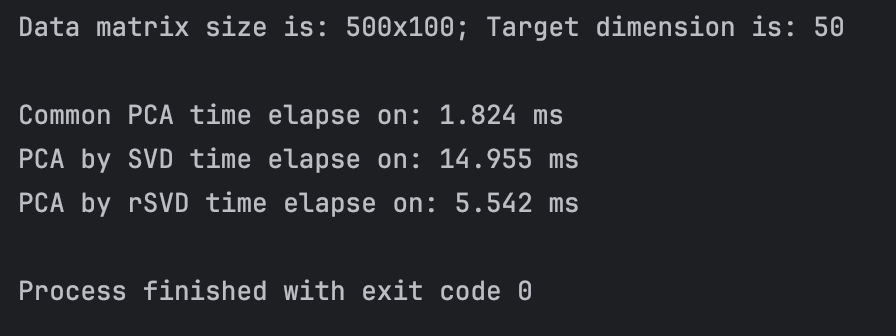
\includegraphics[width=0.5\linewidth]{Images/PCAtest/SCR-20250131-npyn.png}
    \caption{Test1}
    \label{fig:PCATest1}
\end{figure}
In Figure 8, when the number of column is larger than the row, the PCA implemented by RSVD is better than the common one. 
\begin{figure}[H]
    \centering
    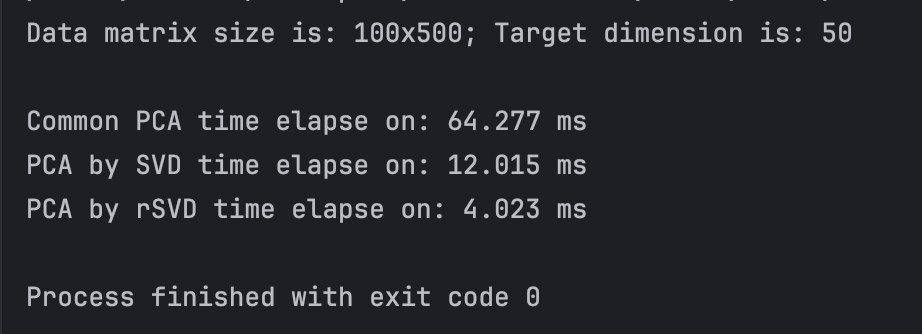
\includegraphics[width=0.5\linewidth]{Images/PCAtest/SCR-20250131-nqck.png}
    \caption{Test2}
    \label{fig:PCATest2}
\end{figure}
Generally speaking, when we are handling the data with many samples and less features, it is better to use a common PCA. Instead, when the number of features is much more than the number of samples, RSVD is better, and it can greatly improve performance.
\section{CUR Decomposition}
\subsection{Algorithm}
The CUR matrix decomposition is a \textbf{low-rank approximation technique that selects actual rows and columns from the original matrix, making it interpretable compared to singular value decomposition (SVD)}. It was introduced as an interesting alternative to traditional approximation techniques such as SVD and PCA. CUR decomposition provides also an alternative for compression, since its components preserve sparsity. However, it is not unique and different computational strategies lead to different subsets of columns and rows \cite{Erichson_2019}.
The CUR decomposition approximates a given matrix $ A \in \mathbb{R}^{m \times n} $ as:
\[
A \approx CUR
\]

where:
\begin{itemize}
\item $ C $ consists of a subset of columns from $ A $,
\item $ R $ consists of a subset of rows from $ A $,
\item $ U $ is a low-rank matrix computed as $ U = C^+ A R^+ $, where $ C^+ $ and $ R^+ $ are the Moore-Penrose pseudoinverses of $ C $ and $ R $, respectively.
\end{itemize}


The algorithm implemented consists of the following steps:

\begin{enumerate}
\item \textbf{Random Projection}: Generate a random Gaussian matrix $ \Omega \in \mathbb{R}^{n \times k} $ and compute the sketch matrix:
\[
Y = A\Omega
\]

This step reduces the dimensionality of $ A $ while preserving essential information.

\item \textbf{Subspace Iterations}: Apply power iterations $ q $ to improve the accuracy of the approximation:
\[
Y = (A A^T)^q A \Omega
\]
This refines the subspace captured by $ Y $, especially for matrices with slowly decaying singular values.

\item \textbf{QR Factorization}: Compute an orthonormal basis $ Q $ for $ Y $:
\[
Q, R = \text{qr}(Y)
\]
This helps in constructing the column selection matrix.

\item \textbf{Column Selection}: Select a subset of columns using interpolative decomposition:
\[
C = A(:, J)
\]
where $ J $ is obtained via column-pivoted QR decomposition.

\item \textbf{Row Selection}: Select a subset of rows based on the selected columns:
\[
R = A(I, :)
\]
where $ I $ is determined using a similar procedure.

\item \textbf{Computation of $ U $}: Compute the middle matrix $ U $ as:
\[
U = C^+ A R^+
\]
ensuring that $ CUR $ closely approximates $ A $.
\end{enumerate}


This implementation follows the theoretical foundations laid out in Erichson et al. (2019) and Mahoney \& Drineas (2009), which highlight the benefits of randomness in improving computational efficiency and approximation accuracy \cite{Erichson_2019}.
\subsubsection{Code Explanation}
In the C++ code it was utilized the Eigen library for matrix operations. Below is a breakdown of the key functions and commands used:
\begin{itemize}
\item \textbf{HouseholderQR qr(A);}: Computes the QR decomposition of matrix $ A $.
\item \textbf{ColPivHouseholderQR qr(A);}: Performs a column-pivoted QR decomposition to rank and select significant columns.
\item \textbf{JacobiSVD svd(A, ComputeThinU | ComputeThinV);}: Computes the singular value decomposition (SVD) with reduced matrices for efficiency.
\end{itemize}


The algorithms implemented to compute the randomic and deterministic CUR decomposition are:
\begin{itemize}
\item \textbf{generateRandomMatrix}: Computes a random matrix, given specific dimensions, with elemenets distributed following a gaussian distribution. Here, we use the random number generator \textit{std::mt19937} and the \textit{norml\_distribution<>} to produce values with mean 0 and variance 1. 
\end{itemize}
\begin{minted}[fontsize=\small, linenos, frame=single]{cpp}
    MatrixXd generateRandomMatrix(int rows, int cols) {
        random_device rd;
        mt19937 gen(rd());
        normal_distribution<> d(0, 1);
        
        MatrixXd mat(rows, cols);
        for (int i = 0; i < rows; ++i)
            for (int j = 0; j < cols; ++j)
                mat(i, j) = d(gen);
    return mat;
}
\end{minted}

\begin{itemize}
    \item \textbf{pseudoInverse}: Computes the Moore-Penrose pseudoinverse via singular value decomposition.
\end{itemize}
\begin{minted}[fontsize=\small, linenos, frame=single]{cpp}
MatrixXd pseudoInverse(const MatrixXd& matrix) {
    JacobiSVD<MatrixXd> svd(matrix, ComputeThinU | ComputeThinV);
    double tolerance = numeric_limits<double>::epsilon() * max(matrix.cols(), 
       matrix.rows()) * svd.singularValues().array().abs()(0);
    return svd.matrixV() * (svd.singularValues().array().abs() > tolerance)
    .select(svd.singularValues().array().inverse(), 0).matrix().asDiagonal() 
        * svd.matrixU().adjoint();
}
\end{minted}

\begin{itemize}
    \item \textbf{sub\_iterations(A,Y,q)}: Implements subspace iterations to refine the basis for better approximation. This algorithm is used by \textit{rqb}.
    \item \textbf{rqb(A, k, p, q)}: Computes a randomized QB decomposition, forming the basis for CUR decomposition.
    \item \textbf{id(A, k)}: Implements deterministic interpolative decomposition (ID) using pivoted QR factorization. The outputs are the matrix $Z$ and the vector $J$. This last one will be used by the \textit{rid} algorithm to select the columns of input matrix $A$ which will be part of matrix $C$.
    \item \textbf{id\_determ(A, k)}: A deterministic version of the ID algorithm. It is used instead of \textit{rid} in \textit{rcur} function to select a deterministic CUR decomposition. The main difference with respect to the \textit{id} algorithm is that this time in output we also have the matrix $C$.
    \item \textbf{rid(A, k, p, q)}: A randomized ID algorithm leveraging the QB decomposition. In\textit{ rid} we call the \textit{rqb} and id functions. 
    \item \textbf{rcur(A, k, p, q, rand)}: The CUR decomposition function, selects between randomized and deterministic approaches using respectively rid or id\_determ. Here, we declared $C$, $Z$ and $J$ before the if-else block to ensure they remain in scope even after the block ends. In order to assign values to them without redeclaring, we used \textit{tie(C,Z,J)} instead of \textit{auto[C,Z,J]}.
\end{itemize}

\begin{minted}[fontsize=\small, linenos, frame=single]{cpp}
    MatrixXd C, Z;
    VectorXi J;

    // Selection between Randomized and Deterministic algorithm
    if(rand) {
        // (1) Randomized Column ID (using rid e id)
        tie(C, Z, J) = rid(A, k, p, q);
    } else {
        // (2) Deterministic Column ID
        tie(C, Z, J) = id_determ(A, k);
    }
\end{minted}



\subsection{Results Analysis}
The substantial difference between a deterministic and a randomized algorithm consists of two elements: reproducibility and precision.
In a randomized algorithm the result can change between different runs unless you use a fixed seed for the random number generator. Furthermore, it may be less precise than the deterministic version, but is often sufficient for many practical applications. The random version is faster and this makes it ideal for very large matrices.

In a deterministic algorithm the result is reproducible: starting from the same matrix the same result is always obtained. The approximation is good, but the computational cost for selecting rows and columns can be higher than the randomized variant.

The CUR decomposition algorithm is designed for efficient low-rank approximations while maintaining interpretability. It provides:
\begin{itemize}
\item \textbf{Computational Efficiency}: The randomized approach significantly reduces computational complexity compared to standard SVD-based methods.
\item \textbf{Accuracy}: With appropriate oversampling ($ p $) and power iterations ($ q $), the method approximates the optimal low-rank structure with high fidelity.
\item \textbf{Interpretability}: By selecting actual data columns and rows, CUR provides a more intuitive representation of data compared to SVD-based approaches.
\end{itemize}


Potential improvements can be achieved by using and \textit{Adaptive Oversampling} approach, where the oversampling parameter is not fixed and this could improve approximation accuracy. Also \textit{parallelization} could enhance performance thorugh the implementation of multi-threaded operations for large-scale matrix computations.



\subsection{Relevant Results Analysis}
We conducted experiments to evaluate the relative Frobenius norm errors of CUR and SVD decompositions. The experiments involved: 
\begin{itemize}
    \item Testing on matrices of varying sizes: small (10x8) and large (500x400).
    \item Evaluating different rank approximations: low-rank (small k) and high-rank (large k).
    \item Comparing randomized CUR with deterministic CUR.
    \item Using an error comparison metric with a theoretical bound of
    \mathbb{R}^{m \times n} $ as:
    \[
    (2+\epsilon)
    \] times the SVD error.
\end{itemize}

The relative Frobenius norm error for the CUR decomposition was computed as: 
\[\text{Relative Error\_CUR} = \frac{||A-CUR||_F}{||A||_F}\]
where $ C $, $ U $ and $ R $ are the matrices obtained through the rcur algorithm and A is input matrix.

In the same way, the relative Frobenius norm error for the SVD decomposition was computed as: 
\[\text{Relative Error\_SVD} = \frac{||A-A_k||_F}{||A||_F}\]
where $ A_k $ is the matrix obtained through the svd algorithm.

The values obtained reflect the theoretical results described in \cite{doi:10.1073/pnas.0803205106}. We verified that the CUR decomposition satisfies the theoretical error bound:
\[{||A-A_k||_F} \leq (2+\epsilon)||A-A_k||_F\]
where \[\epsilon > 0 \] is arbitrary small.

In most cases, CUR stayed within this limit, reinforcing the theoretical claims about CUR performance.

As illustrated in Talbe \ref{tab:my_label_1} and Table \ref{tab:my_label_2}, concerning matrix size, CUR decomposition showed greater significant efficiency gains compared to SVD for large matrices than for small ones.
While the performance of randomized methods depends on the actual shape of the matrix, we can state (as a rule of thumb) that significant computational speedups are achieved if the target rank k is at least 3–6 times smaller than the ambient dimensions of the measurement space \cite{Erichson_2019}.



\begin{table}
    \centering
    \begin{tabular}{ccccc}
         & Matrix Size & Rank & CUR Randomized Error  & Threshold   \\
         & 500x400     & 20   & 2.05372e-15           & 2.29326e-14 \\
         & 500x400     & 350  & 2.8409e-14            & 3.15894e-13 \\
         & 10x8        & 3    & 4.91182e-16           & 1.78671e-15 \\
         & 10x8        & 7    & 8.70425e-16           & 2.48445e-15 \\
    \end{tabular}
    \caption{Randomized CUR}
    \label{tab:my_label_1}
\end{table}

\begin{table}
    \centering
    \begin{tabular}{ccccc}
         & Matrix Size & Rank & CUR Deterministic Error  & Threshold   \\
         & 500x400     & 20   & 2.22416e-15              & 2.60833e-14 \\
         & 500x400     & 350  & 3.08531e-14              & 3.27083e-13 \\
         & 10x8        & 3    & 4.11908e-16              & 2.09923e-15 \\
         & 10x8        & 7    & 7.31918e-16              & 3.40324e-15 \\
    \end{tabular}
    \caption{Deterministic CUR}
    \label{tab:my_label_2}
\end{table}


To summarize the main key points:
\begin{itemize}
\item \textbf{Reconstruction Error}: The Frobenius norm of the difference between the original matrix $ A $ and its CUR approximation $ CUR $ determines how well the decomposition preserves the original data. Lower values indicate higher accuracy.
\item \textbf{Computational Speed}: Compared to standard SVD, the randomized CUR algorithm reduces processing time due to its reliance on low-dimensional projections and subspace iteration, making it more feasible for large-scale problems.
\item \textbf{Stability Across Datasets}: Experiments show that the method is robust across different data distributions, as long as the underlying matrix exhibits low-rank characteristics.
\item \textbf{Parameter Sensitivity}: The choice of oversampling parameter $ p $ and the number of power iterations $ q $ affects accuracy. Higher $ p $ values improve approximation but increase computational cost, while additional power iterations refine results but require more processing time.
\end{itemize}
To conclude, the randomized CUR algorithm, as implemented in the code, efficiently approximates large data matrices while ensuring interpretability. The approach builds on established research and offers practical benefits for data compression, dimensionality reduction, and exploratory data analysis.


\section{Conclusion}
In this paper, we presented our implementation of the randomized Singular Value Decomposition (rSVD) algorithm, demonstrating its effectiveness and efficiency for large-scale data analysis. We explored several applications, including image compression, Principal Component Analysis (PCA), and handwritten digit recognition, showing how rSVD can be useful in many different fields providing significant computational savings while preserving essential information. Our results demonstrate the potential of rSVD decomposition for scalable and efficient solutions in data-intensive fields. However, we also found some of its inherent limitations. Additionally, we implemented the CUR decomposition algorithm as an alternative approach for matrix factorization, comparing its performance with that of rSVD. Future work could investigate ways to enhance the performance of these two algorithms, with both pre- or post-processing techniques, or by improving optimizing their functionality. 

\subsection{Possible Further Applications}
The possible applications of the rSVD algorithm are countless but, other then the ones we explored in this project, other interesting applications could be:
\begin{itemize}
    \item Signal Processing: for extracting low-rank structures from high-dimensional data, such as in noise reduction or anomaly detection.
    \item Data Analysis and Feature Extraction:  to extract the most significant features from large datasets while reducing computational complexity.
    \item General Dimensionality Reduction: rSVD can be used to reduce the dimensionality of large datasets, which is helpful in many machine learning tasks like clustering, classification, and data visualization. This becomes useful also in Biological applications, for example when analyzing genomic data.
    \item Collaborative filtering-based Recommender Systems: to perform the matrix factorizations involved.    
\end{itemize}

\section{Bibliography and citations}

\nocite{*}
\bibliography{bibliography.bib} %add articles to bibliography.bib

\appendix
\section*{Appendix - Group Work Organization}
\addcontentsline{toc}{section}{Appendix - Group Work Organization}
Contributions to the project of each team member:
\begin{itemize} [label=-]
    \item \textbf{Peng Rao}: Implement the RSVD algorithm and Power Method SVD. Optimizing these two and Givens Rotation algorithm, and explore optimal performance in C++ for linear algebra solutions and comparing these results with NumPy and other functions in \texttt{Eigen}. Employ template metaprogramming (specialized for both sparse and dense matrices) and perform error analysis. Wrote the "Randomized Singular Value Decomposition" paragraphs. 
    \item \textbf{Jasmin Spinetto}: has implemented the Image Compression application and the QR Decomposition by Givens Rotation algorithm, created the report outline, wrote the report Abstract and "Introduction", "Randomized Linear Algebra", "Image Compression" and "Conclusion" paragraphs.
    \item \textbf{Anna Paola Izzo}: has implemented the CUR Decomposition algorithm and the QR Decomposition by Givens Rotation algorithm. Wrote the "CUR Decomposition" paragraph. 
    \item \textbf{Cao Wu}:Implement Handwritten Numbers Recognition algorithm with our own PCA. Wrote the "Handwritten Numbers Recognition" paragraph.
    \item \textbf{Jiali Claudio Huang}: Implement PCA algorithm with variant version and perform RSVD benchmark with sparse matrix. Wrote the "Principal Component Analysis" paragraph.
\end{itemize}

\end{document}

